% Options for packages loaded elsewhere
\PassOptionsToPackage{unicode}{hyperref}
\PassOptionsToPackage{hyphens}{url}
%
\documentclass[
]{article}
\usepackage{amsmath,amssymb}
\usepackage{lmodern}
\usepackage{iftex}
\ifPDFTeX
  \usepackage[T1]{fontenc}
  \usepackage[utf8]{inputenc}
  \usepackage{textcomp} % provide euro and other symbols
\else % if luatex or xetex
  \usepackage{unicode-math}
  \defaultfontfeatures{Scale=MatchLowercase}
  \defaultfontfeatures[\rmfamily]{Ligatures=TeX,Scale=1}
\fi
% Use upquote if available, for straight quotes in verbatim environments
\IfFileExists{upquote.sty}{\usepackage{upquote}}{}
\IfFileExists{microtype.sty}{% use microtype if available
  \usepackage[]{microtype}
  \UseMicrotypeSet[protrusion]{basicmath} % disable protrusion for tt fonts
}{}
\makeatletter
\@ifundefined{KOMAClassName}{% if non-KOMA class
  \IfFileExists{parskip.sty}{%
    \usepackage{parskip}
  }{% else
    \setlength{\parindent}{0pt}
    \setlength{\parskip}{6pt plus 2pt minus 1pt}}
}{% if KOMA class
  \KOMAoptions{parskip=half}}
\makeatother
\usepackage{xcolor}
\usepackage{longtable,booktabs,array}
\usepackage{calc} % for calculating minipage widths
% Correct order of tables after \paragraph or \subparagraph
\usepackage{etoolbox}
\makeatletter
\patchcmd\longtable{\par}{\if@noskipsec\mbox{}\fi\par}{}{}
\makeatother
% Allow footnotes in longtable head/foot
\IfFileExists{footnotehyper.sty}{\usepackage{footnotehyper}}{\usepackage{footnote}}
\makesavenoteenv{longtable}
\usepackage{graphicx}
\makeatletter
\def\maxwidth{\ifdim\Gin@nat@width>\linewidth\linewidth\else\Gin@nat@width\fi}
\def\maxheight{\ifdim\Gin@nat@height>\textheight\textheight\else\Gin@nat@height\fi}
\makeatother
% Scale images if necessary, so that they will not overflow the page
% margins by default, and it is still possible to overwrite the defaults
% using explicit options in \includegraphics[width, height, ...]{}
\setkeys{Gin}{width=\maxwidth,height=\maxheight,keepaspectratio}
% Set default figure placement to htbp
\makeatletter
\def\fps@figure{htbp}
\makeatother
\setlength{\emergencystretch}{3em} % prevent overfull lines
\providecommand{\tightlist}{%
  \setlength{\itemsep}{0pt}\setlength{\parskip}{0pt}}
\setcounter{secnumdepth}{-\maxdimen} % remove section numbering
\ifLuaTeX
  \usepackage{selnolig}  % disable illegal ligatures
\fi
\IfFileExists{bookmark.sty}{\usepackage{bookmark}}{\usepackage{hyperref}}
\IfFileExists{xurl.sty}{\usepackage{xurl}}{} % add URL line breaks if available
\urlstyle{same} % disable monospaced font for URLs
\hypersetup{
  hidelinks,
  pdfcreator={LaTeX via pandoc}}

\author{}
\date{}

\begin{document}

\textbf{NEUROSHELL}

An AI System That Fixes Its Own Errors While Running\\
Security Tools on Kali Linux

\emph{Component 3 (AEERE) of the NeuroShell Framework}

\textbf{Project Reference: R26-CS-018}

Final-Year Dissertation

\textbf{Umayanga H.L.A}

IT22230010

B.Sc. (Hons) in Information Technology

Specializing in Cyber Security

Department of Computer Systems Engineering

Sri Lanka Institute of Information Technology

October 2026

\hypertarget{declaration}{%
\section{Declaration}\label{declaration}}

I declare that this dissertation is my own work. It has not been handed
in for any other degree or diploma at this or any other institution.
Where I have used the work or ideas of other people, I have said so in
the text, and the full list of sources is given in the references.

This dissertation is about Component 3 of the NeuroShell group project
(R26-CS-018), which is called the Adaptive Execution and Error-Recovery
Engine. I designed, built and tested this component myself. The other
three components were built by the other members of my group. I mention
their work only where it helps to explain how my part fits in.

\begin{longtable}[]{@{}
  >{\raggedright\arraybackslash}p{(\columnwidth - 4\tabcolsep) * \real{0.3419}}
  >{\raggedright\arraybackslash}p{(\columnwidth - 4\tabcolsep) * \real{0.3376}}
  >{\raggedright\arraybackslash}p{(\columnwidth - 4\tabcolsep) * \real{0.3205}}@{}}
\toprule()
\begin{minipage}[b]{\linewidth}\raggedright
\textbf{Name}
\end{minipage} & \begin{minipage}[b]{\linewidth}\raggedright
\textbf{Signature}
\end{minipage} & \begin{minipage}[b]{\linewidth}\raggedright
\textbf{Date}
\end{minipage} \\
\midrule()
\endhead
Umayanga H.L.A & & \\
\bottomrule()
\end{longtable}

The student named above did this research under my supervision.

\begin{longtable}[]{@{}
  >{\raggedright\arraybackslash}p{(\columnwidth - 4\tabcolsep) * \real{0.3419}}
  >{\raggedright\arraybackslash}p{(\columnwidth - 4\tabcolsep) * \real{0.3376}}
  >{\raggedright\arraybackslash}p{(\columnwidth - 4\tabcolsep) * \real{0.3205}}@{}}
\toprule()
\begin{minipage}[b]{\linewidth}\raggedright
\textbf{Supervisor}
\end{minipage} & \begin{minipage}[b]{\linewidth}\raggedright
\textbf{Signature}
\end{minipage} & \begin{minipage}[b]{\linewidth}\raggedright
\textbf{Date}
\end{minipage} \\
\midrule()
\endhead
Dr. Harinda Fernando & & \\
Mr. Indunil Daluwatte (Co-Supervisor) & & \\
\bottomrule()
\end{longtable}

\hypertarget{abstract}{%
\section{Abstract}\label{abstract}}

Security testers use a long list of command-line tools on Kali Linux,
such as nmap, gobuster, hydra and sqlmap. The problem is that these
tools fail very often. A tool may not be installed, a permission may be
missing, a target may be unreachable, or a command may have a wrong
flag. When this happens, the automated scan simply stops and waits. Even
the newer AI tools like PentestGPT, VulnBot and xOffense do the same
thing: they show the error to the user and give up. A human then has to
read the error, fix the command, and start again. This is the main
reason security scans cannot run on their own from start to finish.

This dissertation builds and tests a system that solves this problem. It
is called the Adaptive Execution and Error-Recovery Engine, or AEERE,
and it is Component 3 of the NeuroShell project. The idea is simple.
Every command runs inside a Docker container with Kali Linux, so nothing
can harm the real computer. If the command fails, the engine reads the
error, works out what went wrong, fixes the command, and tries again,
all by itself. To work out what went wrong, it uses three steps one
after another: a fast pattern check, a text-similarity check, and
finally a local AI model (Gemma, run through Ollama) that reasons about
the error. Before any fixed command is allowed to run, it must pass
three safety checks. Because the AI runs on the same computer, no
command or error or target is ever sent to the internet.

The engine was tested on a dataset I built of 8,000 real failure cases.
These cover ten kinds of errors, more than eighteen tools, and three
difficulty levels. The tests measure how often the engine fixes the
error, how accurately it labels the error type, how fast it is, how much
computer power it uses, and whether it ever lets a dangerous command
through. The full engine is compared against two simpler methods. The
targets are a fix rate of at least 80\%, an error-labelling score above
90\%, a full fix attempt within ten seconds, and zero dangerous commands
getting through.

\textbf{Keywords ---} \emph{error recovery; local AI language model;
automated penetration testing; self-healing system; Kali Linux; command
fixing; sandboxed execution.}

\hypertarget{acknowledgement}{%
\section{Acknowledgement}\label{acknowledgement}}

I want to thank my supervisor, Dr. Harinda Fernando, and my
co-supervisor, Mr. Indunil Daluwatte, for their help and patience during
this project. Their feedback helped me decide the direction of the work
and made this report clearer.

I also thank the lecturers at the Faculty of Computing at SLIIT for the
knowledge and the support that made this work possible.

Thanks also go to my group members, who built the other three parts of
NeuroShell. Their progress on the other parts helped me understand
exactly what my component had to do.

Finally, I thank my family and friends for supporting me throughout my
studies.

\hypertarget{table-of-contents}{%
\section{Table of Contents}\label{table-of-contents}}

\protect\hyperlink{declaration}{Declaration
\protect\hyperlink{declaration}{1}}

\protect\hyperlink{abstract}{Abstract \protect\hyperlink{abstract}{1}}

\protect\hyperlink{acknowledgement}{Acknowledgement
\protect\hyperlink{acknowledgement}{1}}

\protect\hyperlink{table-of-contents}{Table of Contents
\protect\hyperlink{table-of-contents}{1}}

\protect\hyperlink{list-of-figures}{List of Figures
\protect\hyperlink{list-of-figures}{1}}

\protect\hyperlink{list-of-tables}{List of Tables
\protect\hyperlink{list-of-tables}{1}}

\protect\hyperlink{list-of-abbreviations}{List of Abbreviations
\protect\hyperlink{list-of-abbreviations}{1}}

\protect\hyperlink{introduction}{1 Introduction
\protect\hyperlink{introduction}{1}}

\protect\hyperlink{background}{1.1 Background
\protect\hyperlink{background}{1}}

\protect\hyperlink{the-real-problem}{1.1.1 The Real Problem
\protect\hyperlink{the-real-problem}{1}}

\protect\hyperlink{who-this-affects}{1.1.2 Who This Affects
\protect\hyperlink{who-this-affects}{1}}

\protect\hyperlink{some-numbers}{1.1.3 Some Numbers
\protect\hyperlink{some-numbers}{1}}

\protect\hyperlink{current-solutions-and-their-limits}{1.1.4 Current
Solutions and Their Limits
\protect\hyperlink{current-solutions-and-their-limits}{1}}

\protect\hyperlink{the-proposed-solution}{1.1.5 The Proposed Solution
\protect\hyperlink{the-proposed-solution}{1}}

\protect\hyperlink{link-to-the-un-sustainable-development-goals}{1.1.6
Link to the UN Sustainable Development Goals
\protect\hyperlink{link-to-the-un-sustainable-development-goals}{1}}

\protect\hyperlink{research-cluster}{1.1.7 Research Cluster
\protect\hyperlink{research-cluster}{1}}

\protect\hyperlink{the-research-problem}{1.2 The Research Problem
\protect\hyperlink{the-research-problem}{1}}

\protect\hyperlink{literature-review-and-objectives}{2 Literature Review
and Objectives \protect\hyperlink{literature-review-and-objectives}{1}}

\protect\hyperlink{how-self-correcting-ai-agents-grew}{2.1 How
Self-Correcting AI Agents Grew
\protect\hyperlink{how-self-correcting-ai-agents-grew}{1}}

\protect\hyperlink{how-other-security-ai-systems-handle-errors}{2.2 How
Other Security AI Systems Handle Errors
\protect\hyperlink{how-other-security-ai-systems-handle-errors}{1}}

\protect\hyperlink{comparing-existing-systems}{2.3 Comparing Existing
Systems \protect\hyperlink{comparing-existing-systems}{1}}

\protect\hyperlink{the-research-gap}{2.4 The Research Gap
\protect\hyperlink{the-research-gap}{1}}

\protect\hyperlink{objectives}{2.5 Objectives
\protect\hyperlink{objectives}{1}}

\protect\hyperlink{main-objective}{2.5.1 Main Objective
\protect\hyperlink{main-objective}{1}}

\protect\hyperlink{specific-objectives}{2.5.2 Specific Objectives
\protect\hyperlink{specific-objectives}{1}}

\protect\hyperlink{methodology-and-system-design}{3 Methodology and
System Design \protect\hyperlink{methodology-and-system-design}{1}}

\protect\hyperlink{research-approach}{3.1 Research Approach
\protect\hyperlink{research-approach}{1}}

\protect\hyperlink{how-the-whole-system-works}{3.2 How the Whole System
Works \protect\hyperlink{how-the-whole-system-works}{1}}

\protect\hyperlink{how-component-3-works-the-five-stages}{3.3 How
Component 3 Works: The Five Stages
\protect\hyperlink{how-component-3-works-the-five-stages}{1}}

\protect\hyperlink{stage-1---run-the-command}{Stage 1 --- Run the
Command \protect\hyperlink{stage-1---run-the-command}{1}}

\protect\hyperlink{stage-2---label-the-error}{Stage 2 --- Label the
Error \protect\hyperlink{stage-2---label-the-error}{1}}

\protect\hyperlink{stage-3---work-out-the-cause}{Stage 3 --- Work Out
the Cause \protect\hyperlink{stage-3---work-out-the-cause}{1}}

\protect\hyperlink{stage-4---fix-and-check}{Stage 4 --- Fix and Check
\protect\hyperlink{stage-4---fix-and-check}{1}}

\protect\hyperlink{stage-5---retry-or-stop-nicely}{Stage 5 --- Retry or
Stop Nicely \protect\hyperlink{stage-5---retry-or-stop-nicely}{1}}

\protect\hyperlink{the-three-step-error-check}{3.4 The Three-Step Error
Check \protect\hyperlink{the-three-step-error-check}{1}}

\protect\hyperlink{the-error-list}{3.5 The Error List
\protect\hyperlink{the-error-list}{1}}

\protect\hyperlink{building-the-test-dataset}{3.6 Building the Test
Dataset \protect\hyperlink{building-the-test-dataset}{1}}

\protect\hyperlink{tools-used-and-why}{3.7 Tools Used and Why
\protect\hyperlink{tools-used-and-why}{1}}

\protect\hyperlink{how-the-engine-is-tested}{3.8 How the Engine Is
Tested \protect\hyperlink{how-the-engine-is-tested}{1}}

\protect\hyperlink{how-it-was-built}{4 How It Was Built
\protect\hyperlink{how-it-was-built}{1}}

\protect\hyperlink{the-data-model}{4.1 The Data Model
\protect\hyperlink{the-data-model}{1}}

\protect\hyperlink{the-sandboxed-command-runner}{4.2 The Sandboxed
Command Runner \protect\hyperlink{the-sandboxed-command-runner}{1}}

\protect\hyperlink{catching-and-cleaning-the-error}{4.3 Catching and
Cleaning the Error
\protect\hyperlink{catching-and-cleaning-the-error}{1}}

\protect\hyperlink{the-three-step-error-check-1}{4.4 The Three-Step
Error Check \protect\hyperlink{the-three-step-error-check-1}{1}}

\protect\hyperlink{the-fix-engine}{4.5 The Fix Engine
\protect\hyperlink{the-fix-engine}{1}}

\protect\hyperlink{the-safety-check}{4.6 The Safety Check
\protect\hyperlink{the-safety-check}{1}}

\protect\hyperlink{retries-and-logging}{4.7 Retries and Logging
\protect\hyperlink{retries-and-logging}{1}}

\protect\hyperlink{session-memory}{4.8 Session Memory
\protect\hyperlink{session-memory}{1}}

\protect\hyperlink{putting-it-together-and-deploying}{4.9 Putting It
Together and Deploying
\protect\hyperlink{putting-it-together-and-deploying}{1}}

\protect\hyperlink{results-and-testing}{5 Results and Testing
\protect\hyperlink{results-and-testing}{1}}

\protect\hyperlink{test-setup}{5.1 Test Setup
\protect\hyperlink{test-setup}{1}}

\protect\hyperlink{fix-rate-so3---to-be-measured-on-the-live-engine}{5.2
Fix Rate (SO3) --- to be measured on the live engine
\protect\hyperlink{fix-rate-so3---to-be-measured-on-the-live-engine}{1}}

\protect\hyperlink{error-labelling-accuracy-so3-measured}{5.3
Error-Labelling Accuracy (SO3) --- measured
\protect\hyperlink{error-labelling-accuracy-so3-measured}{1}}

\protect\hyperlink{speed-and-cost-so4}{5.4 Speed and Cost (SO4)
\protect\hyperlink{speed-and-cost-so4}{1}}

\protect\hyperlink{safety-test-so5-to-be-measured-on-the-live-engine}{5.5
Safety Test (SO5) --- to be measured on the live engine
\protect\hyperlink{safety-test-so5-to-be-measured-on-the-live-engine}{1}}

\protect\hyperlink{average-tries-to-succeed-so3---to-be-measured-on-the-live-engine}{5.6
Average Tries to Succeed (SO3) --- to be measured on the live engine
\protect\hyperlink{average-tries-to-succeed-so3---to-be-measured-on-the-live-engine}{1}}

\protect\hyperlink{summary-of-results}{5.7 Summary of Results
\protect\hyperlink{summary-of-results}{1}}

\protect\hyperlink{discussion-conclusion-and-future-work}{6 Discussion,
Conclusion and Future Work
\protect\hyperlink{discussion-conclusion-and-future-work}{1}}

\protect\hyperlink{discussion}{6.1 Discussion
\protect\hyperlink{discussion}{1}}

\protect\hyperlink{limits}{6.2 Limits \protect\hyperlink{limits}{1}}

\protect\hyperlink{future-work}{6.3 Future Work
\protect\hyperlink{future-work}{1}}

\protect\hyperlink{conclusion}{6.4 Conclusion
\protect\hyperlink{conclusion}{1}}

\protect\hyperlink{references}{References
\protect\hyperlink{references}{1}}

\protect\hyperlink{appendices}{Appendices
\protect\hyperlink{appendices}{1}}

\protect\hyperlink{appendix-a---full-error-list}{Appendix A --- Full
Error List \protect\hyperlink{appendix-a---full-error-list}{1}}

\protect\hyperlink{appendix-b--api-reference}{Appendix B --- API
Reference \protect\hyperlink{appendix-b--api-reference}{1}}

\protect\hyperlink{appendix-c---sample-test-cases}{Appendix C --- Sample
Test Cases \protect\hyperlink{appendix-c---sample-test-cases}{1}}

\protect\hyperlink{appendix-d---ethics-and-risk}{Appendix D --- Ethics
and Risk \protect\hyperlink{appendix-d---ethics-and-risk}{1}}

\hypertarget{list-of-figures}{%
\section{List of Figures}\label{list-of-figures}}

Figure 1. The four parts of NeuroShell Ch. 3

Figure 2. How Component 3 fixes an error (the loop) Ch. 3

Figure 3. The three-step error check Ch. 4

Figure 4. The 8,000 test cases by error type Ch. 3

Figure 5. Labelling accuracy as message noise rises Ch. 5

Figure 6. Confusion matrix at 30\% message noise Ch. 5

\hypertarget{list-of-tables}{%
\section{List of Tables}\label{list-of-tables}}

Table 1. Comparison of existing AI security tools Ch. 2

Table 2. Weaknesses of current automated testing systems Ch. 2

Table 3. The four NeuroShell parts and what is new about each Ch. 2

Table 4. The eight error types and how each is fixed Ch. 3

Table 5. The test dataset at a glance Ch. 3

Table 6. Tools used and why Ch. 3

Table 7. What each test measures Ch. 3

Table 8. Fix rate by method (live engine) Ch. 5

Table 9. Labelling accuracy as message noise rises Ch. 5

Table 10. Accuracy for each error type at 30\% noise Ch. 5

Table 11. Speed by step Ch. 5

Table 12. Dangerous-command block rate (live engine) Ch. 5

\hypertarget{list-of-abbreviations}{%
\section{List of Abbreviations}\label{list-of-abbreviations}}

\begin{longtable}[]{@{}
  >{\raggedright\arraybackslash}p{(\columnwidth - 2\tabcolsep) * \real{0.2778}}
  >{\raggedright\arraybackslash}p{(\columnwidth - 2\tabcolsep) * \real{0.7222}}@{}}
\toprule()
\begin{minipage}[b]{\linewidth}\raggedright
\textbf{Short form}
\end{minipage} & \begin{minipage}[b]{\linewidth}\raggedright
\textbf{Meaning}
\end{minipage} \\
\midrule()
\endhead
AEERE & Adaptive Execution and Error-Recovery Engine (Component 3) \\
API & Application Programming Interface \\
CVE & Common Vulnerabilities and Exposures \\
DSR & Design Science Research \\
F1 & F1-Score (a measure of labelling accuracy) \\
JSON & JavaScript Object Notation \\
LLM & Large Language Model (AI language model) \\
NLU & Natural Language Understanding \\
RAG & Retrieval-Augmented Generation \\
RFC-1918 & Private IP address ranges used inside local networks \\
SOC & Security Operations Centre \\
stderr / stdout & Error output / Normal output of a command \\
TTL & Time To Live \\
\bottomrule()
\end{longtable}

\hypertarget{introduction}{%
\section{1 Introduction}\label{introduction}}

\hypertarget{background}{%
\subsection{1.1 Background}\label{background}}

\hypertarget{the-real-problem}{%
\subsubsection{1.1.1 The Real Problem}\label{the-real-problem}}

Security testers use tools to scan computers and networks for weak
points. Tools like nmap, gobuster, gobuster run on Kali Linux, and
almost every penetration test uses them. The trouble is that these tools
fail a lot. Sometimes a tool is not installed. Sometimes the user does
not have enough permission. Sometimes the target cannot be reached, or a
flag in the command is wrong. When one command in a chain fails, the
whole scan stops. A person then has to read the error, fix the command
by hand, and start the scan again.

This is a real problem because errors happen all the time in security
work. Today\textquotesingle s tools are not smart enough to fix their
own mistakes. This project solves that. It builds a system where an AI
reads the error, works out what went wrong, and writes a corrected
command on its own, with no human help.

\hypertarget{who-this-affects}{%
\subsubsection{1.1.2 Who This Affects}\label{who-this-affects}}

This problem affects everyone who uses automated security testing. Large
company security teams (SOC teams) lose time every time a scan stops,
which can leave a weakness open for longer. Junior analysts, who already
find these tools hard, are stuck when automation fails and have to ask a
senior person for help. Researchers also suffer, because they have to
watch over every test, which makes large experiments very hard to run.

\hypertarget{some-numbers}{%
\subsubsection{1.1.3 Some Numbers}\label{some-numbers}}

In 2024, researchers found 40,009 new software weaknesses (CVEs). That
is about 38\% more than the year before. At the same time, the world was
short of around 4.8 million cybersecurity workers. So there are far too
many problems and far too few people to deal with them. Automation is
the only way to keep up, but it is only useful if it does not stop every
time a tool shows an error.

\hypertarget{current-solutions-and-their-limits}{%
\subsubsection{1.1.4 Current Solutions and Their
Limits}\label{current-solutions-and-their-limits}}

Older automation used fixed scripts that just crashed when a tool
failed. Newer AI tools like PentestGPT, VulnBot and xOffense are much
better at planning and writing commands, but they all have the same weak
point. When a command fails while running, they stop and show the error
to the user. None of them can work out why the command failed and fix
it. In short, they do not try to understand the error, they cannot swap
one tool for another when the first keeps failing, and they do not use
AI reasoning to find the real cause.

\hypertarget{the-proposed-solution}{%
\subsubsection{1.1.5 The Proposed
Solution}\label{the-proposed-solution}}

This project builds the Adaptive Execution and Error-Recovery Engine
(AEERE), which is one part of the NeuroShell system. Its job is easy to
describe. When a security tool fails, instead of stopping and asking a
human, the engine uses a local AI model to read the error, find the
cause, and write a fixed command to try again. All of this happens
automatically, on the same computer, so no private data leaves the
machine.

\hypertarget{link-to-the-un-sustainable-development-goals}{%
\subsubsection{1.1.6 Link to the UN Sustainable Development
Goals}\label{link-to-the-un-sustainable-development-goals}}

This work supports SDG 9 (Industry, Innovation and Infrastructure) by
making digital security more reliable. It supports SDG 8 (Decent Work
and Economic Growth) by making security testing cheaper and easier for
smaller companies. It also supports SDG 4 (Quality Education), because
it lowers the skill needed, so junior analysts can do tasks that would
normally need an expert.

\hypertarget{research-cluster}{%
\subsubsection{1.1.7 Research Cluster}\label{research-cluster}}

This project belongs to the Information Assurance and Security (IAS)
cluster at SLIIT. It adds to the study of smart, agent-based systems for
automatic vulnerability testing, using AI to manage command execution
and to fix errors on its own.

\hypertarget{the-research-problem}{%
\subsection{1.2 The Research Problem}\label{the-research-problem}}

Security tools fail all the time in real life. When they fail,
today\textquotesingle s AI systems stop and wait for a human. This
project asks one clear question - can we build a system that reads the
error, understands what went wrong, and writes a fixed command by
itself, for the many tools on Kali Linux? No existing tool does this.
This project builds and tests such a system for the first time.

\hypertarget{literature-review-and-objectives}{%
\section{2 Literature Review and
Objectives}\label{literature-review-and-objectives}}

\hypertarget{how-self-correcting-ai-agents-grew}{%
\subsection{2.1 How Self-Correcting AI Agents
Grew}\label{how-self-correcting-ai-agents-grew}}

Early work on AI agents showed that they do better when they can look at
what happened after each action, think about it, and then decide the
next step. The ReAct framework (2023) showed that an AI that mixes
thinking and acting does better than one that only thinks. The Reflexion
framework (2023) went further. When the AI fails a task, it writes a
short note about what went wrong, saves it, and reads it on the next
try. This improved its results on coding and reasoning tasks. The CRITIC
framework (2024) showed that an AI corrects itself better when it looks
at the real output of a tool instead of guessing from memory.

\hypertarget{how-other-security-ai-systems-handle-errors}{%
\subsection{2.2 How Other Security AI Systems Handle
Errors}\label{how-other-security-ai-systems-handle-errors}}

PentestGPT was one of the first big AI security assistants. It tells the
user what command to type, but the user has to run it and paste the
result back. It cannot run commands or fix errors on its own.
AutoAttacker can run commands by itself, but it struggles with tools it
has not seen before and has no error recovery. VulnBot uses several AI
agents that work together, one plans, one scans, one attacks, but when
something fails it just passes the problem up to a manager agent that
does not know how to fix it. xOffense got good results, but only because
it was trained on specific tools. When a tool version changes, it
breaks, because it cannot adapt without training again.

\hypertarget{comparing-existing-systems}{%
\subsection{2.3 Comparing Existing
Systems}\label{comparing-existing-systems}}

\begin{longtable}[]{@{}
  >{\raggedright\arraybackslash}p{(\columnwidth - 6\tabcolsep) * \real{0.2244}}
  >{\raggedright\arraybackslash}p{(\columnwidth - 6\tabcolsep) * \real{0.2671}}
  >{\raggedright\arraybackslash}p{(\columnwidth - 6\tabcolsep) * \real{0.2350}}
  >{\raggedright\arraybackslash}p{(\columnwidth - 6\tabcolsep) * \real{0.2735}}@{}}
\toprule()
\begin{minipage}[b]{\linewidth}\raggedright
\textbf{System}
\end{minipage} & \begin{minipage}[b]{\linewidth}\raggedright
\textbf{How it works}
\end{minipage} & \begin{minipage}[b]{\linewidth}\raggedright
\textbf{What it can do}
\end{minipage} & \begin{minipage}[b]{\linewidth}\raggedright
\textbf{Main weakness}
\end{minipage} \\
\midrule()
\endhead
PentestGPT & Suggests commands for the user to run by hand & Much better
than the base model on test tasks & User runs every command by hand; no
error recovery \\
AutoAttacker & Runs follow-up commands automatically & Runs commands
after breaking into a system & Makes mistakes on new tools; no error
recovery \\
xOffense & Several agents trained on specific tools & Finishes most
sub-tasks & Cannot handle new tool versions without retraining \\
VulnBot & Several agents split across scan, plan, attack & Good at
splitting a big task into smaller ones & Failures are passed to a
manager that cannot fix them \\
\bottomrule()
\end{longtable}

\emph{Table 1. Comparison of existing AI-based security testing tools}

\hypertarget{the-research-gap}{%
\subsection{2.4 The Research Gap}\label{the-research-gap}}

Every system above stops working properly the moment a tool fails while
running. None of them has a part whose only job is to read the error,
understand it, and fix it automatically. This missing part is the gap
that my project fills. The main limits of current tools are listed
below.

\begin{longtable}[]{@{}
  >{\raggedright\arraybackslash}p{(\columnwidth - 4\tabcolsep) * \real{0.2671}}
  >{\raggedright\arraybackslash}p{(\columnwidth - 4\tabcolsep) * \real{0.3526}}
  >{\raggedright\arraybackslash}p{(\columnwidth - 4\tabcolsep) * \real{0.3803}}@{}}
\toprule()
\begin{minipage}[b]{\linewidth}\raggedright
\textbf{Problem}
\end{minipage} & \begin{minipage}[b]{\linewidth}\raggedright
\textbf{What it means}
\end{minipage} & \begin{minipage}[b]{\linewidth}\raggedright
\textbf{Why it is bad}
\end{minipage} \\
\midrule()
\endhead
No error understanding & The system does not try to read the error; it
ignores it or passes it on as plain text & Without understanding the
error, it cannot pick the right fix \\
No cause finding & No attempt to find why the command failed (missing
tool? wrong password? network?) & The fix becomes a random guess, so it
rarely works \\
No tool switching & If one tool keeps failing, no other tool is tried
for the same job & The scan gets stuck on one failing tool even when
another would work \\
Run and forget & Commands run and the system moves on without checking
they worked & Silent failures build up and later steps give wrong
results \\
\bottomrule()
\end{longtable}

\emph{Table 2. Main weaknesses of current automated testing systems}

The Score study (2024) backs up my approach. It found that AI systems
that fix their own mistakes using real output did 15.6\% better on maths
and 9.1\% better on coding. In other words, giving the AI real output to
reason about, instead of letting it guess, gives clearly better fixes.
That is exactly the idea my engine is built on.

\hypertarget{objectives}{%
\subsection{2.5 Objectives}\label{objectives}}

\hypertarget{main-objective}{%
\subsubsection{2.5.1 Main Objective}\label{main-objective}}

To design, build and test a self-healing execution layer that runs
offensive-security commands safely in a sandbox and then finds and fixes
command failures on its own, with no human help.

\hypertarget{specific-objectives}{%
\subsubsection{2.5.2 Specific Objectives}\label{specific-objectives}}

\begin{enumerate}
\def\labelenumi{\arabic{enumi}.}
\item
  SO1
\end{enumerate}

\begin{quote}
Catch failed commands and their error messages and put them into a
clean, organised form the system can read.
\end{quote}

\begin{enumerate}
\def\labelenumi{\arabic{enumi}.}
\setcounter{enumi}{1}
\item
  SO2
\end{enumerate}

\begin{quote}
Run the tools inside a safe, isolated space that records all output, and
start the fixing process automatically when a command fails.
\end{quote}

\begin{enumerate}
\def\labelenumi{\arabic{enumi}.}
\setcounter{enumi}{2}
\item
  SO3
\end{enumerate}

\begin{quote}
Add a local AI model that reads the error, finds the cause, and suggests
a fixed command that is checked before use (target fix rate 80\% or
more; labelling score above 90\%).
\end{quote}

\begin{enumerate}
\def\labelenumi{\arabic{enumi}.}
\setcounter{enumi}{3}
\item
  SO4
\end{enumerate}

\begin{quote}
Measure how fast and how cheaply the engine fixes errors, and compare it
against two simpler methods.
\end{quote}

\begin{enumerate}
\def\labelenumi{\arabic{enumi}.}
\setcounter{enumi}{4}
\item
  SO5
\end{enumerate}

\begin{quote}
Spot cases where the AI suggests a wrong or dangerous command, and add
safety checks so no dangerous command ever runs.
\end{quote}

The table below shows what each NeuroShell part does and what is new
about it, and where my component fits.

\begin{longtable}[]{@{}
  >{\raggedright\arraybackslash}p{(\columnwidth - 4\tabcolsep) * \real{0.2457}}
  >{\raggedright\arraybackslash}p{(\columnwidth - 4\tabcolsep) * \real{0.4551}}
  >{\raggedright\arraybackslash}p{(\columnwidth - 4\tabcolsep) * \real{0.2991}}@{}}
\toprule()
\begin{minipage}[b]{\linewidth}\raggedright
\textbf{Component}
\end{minipage} & \begin{minipage}[b]{\linewidth}\raggedright
\textbf{What it does}
\end{minipage} & \begin{minipage}[b]{\linewidth}\raggedright
\textbf{What is new about it}
\end{minipage} \\
\midrule()
\endhead
C1 -Intent Recognition Engine & Turns plain-English requests into
structured JSON, pulling out IPs, CVEs, ports and schedules & Reads
tricky security wording and removes confusion about what the user
means \\
C2 -Dynamic Planner \& RAG Engine & Reads Linux manuals and tool docs in
real time to build valid commands & Can use tools it has never seen
before, without extra training \\
C3 - AEERE (my work) & Catches errors, labels them, works out the cause,
and fixes the command to try again & First error list built just for
Kali tools, plus swapping one failing tool for another \\
C4 -Vulnerability Analysis Engine & Reads the output logs, finds
weaknesses, and predicts how exploitable they are & Predicts risk and
sends the important findings back to the planner \\
\bottomrule()
\end{longtable}

\emph{Table 3. The four NeuroShell parts and what is new about each}

\hypertarget{methodology-and-system-design}{%
\section{3 Methodology and System
Design}\label{methodology-and-system-design}}

\hypertarget{research-approach}{%
\subsection{3.1 Research Approach}\label{research-approach}}

This project uses the Design Science Research (DSR) method. This method
suits computer science projects where the goal is to build something new
and show that it works. Instead of only studying a problem in theory,
you build a real working system and test it. The work has four steps.
First, understand the problem through the literature review in Chapter
2, which shows that no current system fixes tool errors on its own.
Second, build the engine with all five of its stages. Third, test the
engine on the dataset and measure fix rate, speed, cost and safety.
Fourth, write down the design choices, the results and the findings in
this report.

\hypertarget{how-the-whole-system-works}{%
\subsection{3.2 How the Whole System
Works}\label{how-the-whole-system-works}}

NeuroShell lets a user type a security task in plain English, for
example ``check the web server at 10.0.0.5 for hidden folders'', and the
system does the rest. It has four parts that work as a chain. Each part
is a separate project, and they talk to each other using JSON and share
state through Redis. Figure 1 shows the whole chain and where my part
sits.

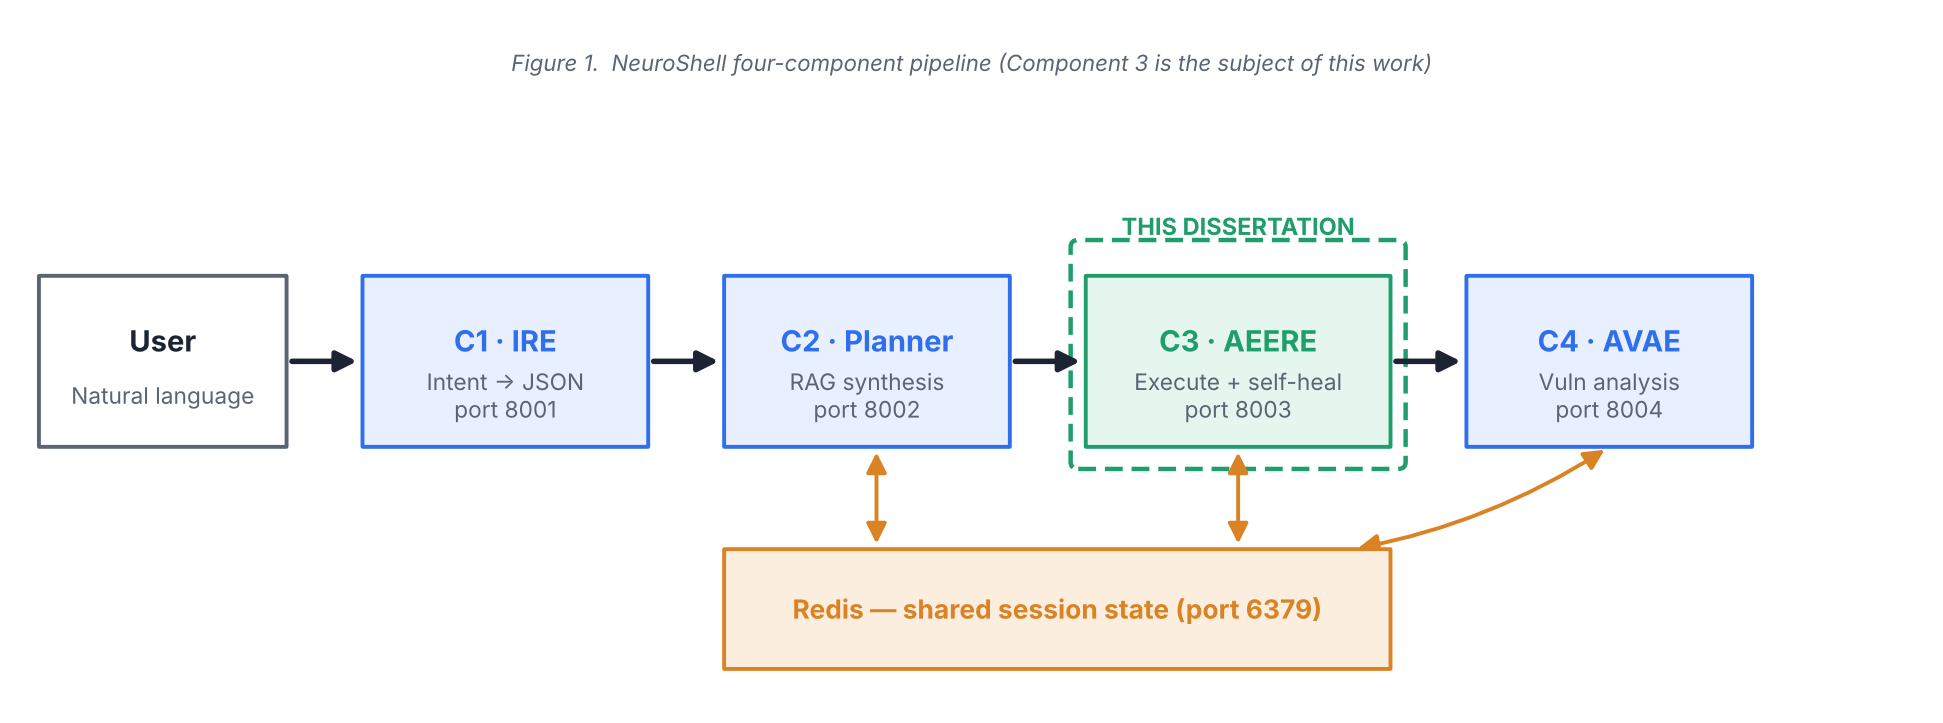
\includegraphics[width=6.25in,height=2.29167in]{vertopal_05e97fad080746c9b767567e93f99da6/media/image1.png}

\emph{Figure 1. The four parts of NeuroShell. Component 3 (AEERE) is the
subject of this report.}

\begin{longtable}[]{@{}
  >{\raggedright\arraybackslash}p{(\columnwidth - 2\tabcolsep) * \real{0.2457}}
  >{\raggedright\arraybackslash}p{(\columnwidth - 2\tabcolsep) * \real{0.7543}}@{}}
\toprule()
\begin{minipage}[b]{\linewidth}\raggedright
\textbf{Component}
\end{minipage} & \begin{minipage}[b]{\linewidth}\raggedright
\textbf{Job}
\end{minipage} \\
\midrule()
\endhead
C1 - Intent Recognition Engine & Reads the plain-English request and
turns it into structured JSON with the intent and the details (port
8001). \\
C2 - Dynamic Planner & Turns the intent into a real command by reading a
store of tool documentation (port 8002). \\
C3 - AEERE & Runs the command in a sandbox, records the output and
errors, and fixes failures on its own (port 8003). \\
C4 -Vulnerability Analysis Engine & Takes the logs from C3, finds
weaknesses, and predicts how risky they are (port 8004). \\
\bottomrule()
\end{longtable}

\emph{Table 4a. The four parts of NeuroShell}

\hypertarget{how-component-3-works-the-five-stages}{%
\subsection{3.3 How Component 3 Works: The Five
Stages}\label{how-component-3-works-the-five-stages}}

My engine works in five stages that form a loop, shown in Figure 2. It
runs a command, and only if it fails do the fixing stages start. A fixed
command goes back to Stage 1 to run again, and this repeats until the
command works or the retry limit for that error type is reached.

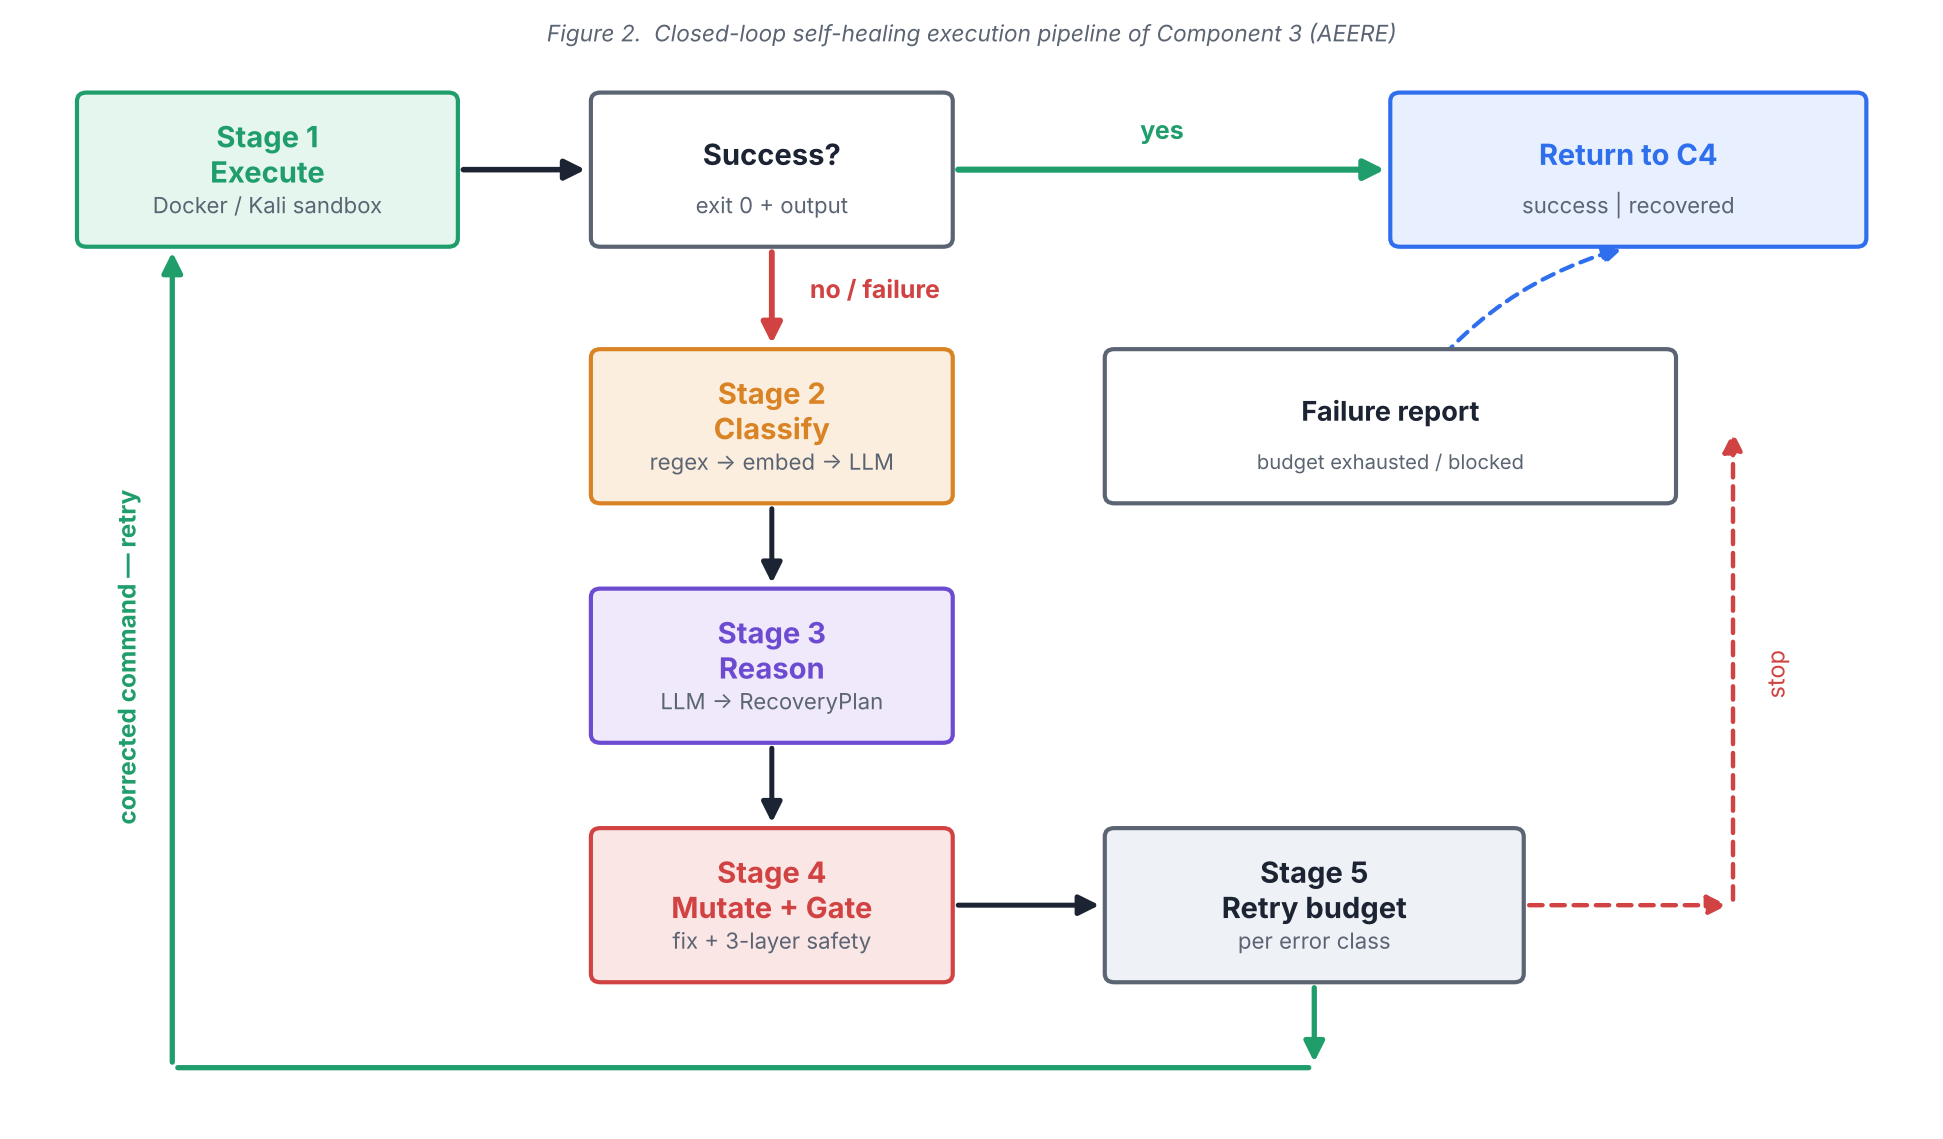
\includegraphics[width=6.25in,height=3.64583in]{vertopal_05e97fad080746c9b767567e93f99da6/media/image2.png}

\emph{Figure 2. How Component 3 fixes an error. The loop keeps trying
until the command works or the retry limit is reached.}

\hypertarget{stage-1---run-the-command}{%
\subsubsection{Stage 1 - Run the
Command}\label{stage-1---run-the-command}}

The command from the Planner goes into a fresh Docker container running
Kali Linux. The container runs the command and records the normal output
and the error output separately, along with the exit code. If the
command works cleanly (exit code 0 with real output), the result is
passed straight on. The fixing stages only start when something goes
wrong. This includes a silent failure, where a tool exits with code 0
but produces no useful output.

\hypertarget{stage-2---label-the-error}{%
\subsubsection{Stage 2 - Label the
Error}\label{stage-2---label-the-error}}

The error is labelled using three steps in order (see Section 3.4). A
fast pattern check runs first, in under 50 milliseconds. If it cannot
label the error, a text-similarity check runs next. Only if both of
those miss does the local AI model run. The first step that works stops
the slower ones, so simple errors stay cheap and fast.

\hypertarget{stage-3---work-out-the-cause}{%
\subsubsection{Stage 3 - Work Out the
Cause}\label{stage-3---work-out-the-cause}}

When the fast steps cannot handle the error, the local AI model gets a
clear prompt with the original command, the full error message, the exit
code, the possible error type, and some context about the task. It
replies with a small JSON plan that has the cause, the chosen fix, and a
corrected command. The reply is checked against a strict format before
the engine goes on. This stage is the main new idea. No existing
security tool uses a local AI to reason about and fix its own errors
like this.

\hypertarget{stage-4---fix-and-check}{%
\subsubsection{Stage 4 - Fix and Check}\label{stage-4---fix-and-check}}

Based on the cause, the engine applies one fix: install the missing
tool, add sudo, change the settings, swap in a different tool, or
rewrite the command. Before the fixed command runs, it must pass three
safety checks: a format check, a dangerous-word check, and a
confidence-and-scope check (see Section 3.5). Only commands that pass
all three go back to Stage 1.

\hypertarget{stage-5---retry-or-stop-nicely}{%
\subsubsection{Stage 5 - Retry or Stop
Nicely}\label{stage-5---retry-or-stop-nicely}}

Each error type has a retry limit and a wait rule. For example, network
errors can be tried up to three times with a growing wait between tries.
If the limit is reached, the engine writes a clear report that says what
it tried and why it did not work, and then stops. The retry limit makes
sure the engine can never get stuck in a loop forever.

\hypertarget{the-three-step-error-check}{%
\subsection{3.4 The Three-Step Error
Check}\label{the-three-step-error-check}}

Labelling the error is the key step, because the error type decides the
fix. Three steps, shown in Figure 3, trade speed against thinking power.
Simple, common errors are handled at once by pattern matching. Unusual
or mixed errors go to the AI. Anything the AI cannot handle is marked
UNKNOWN and sent out of the loop.

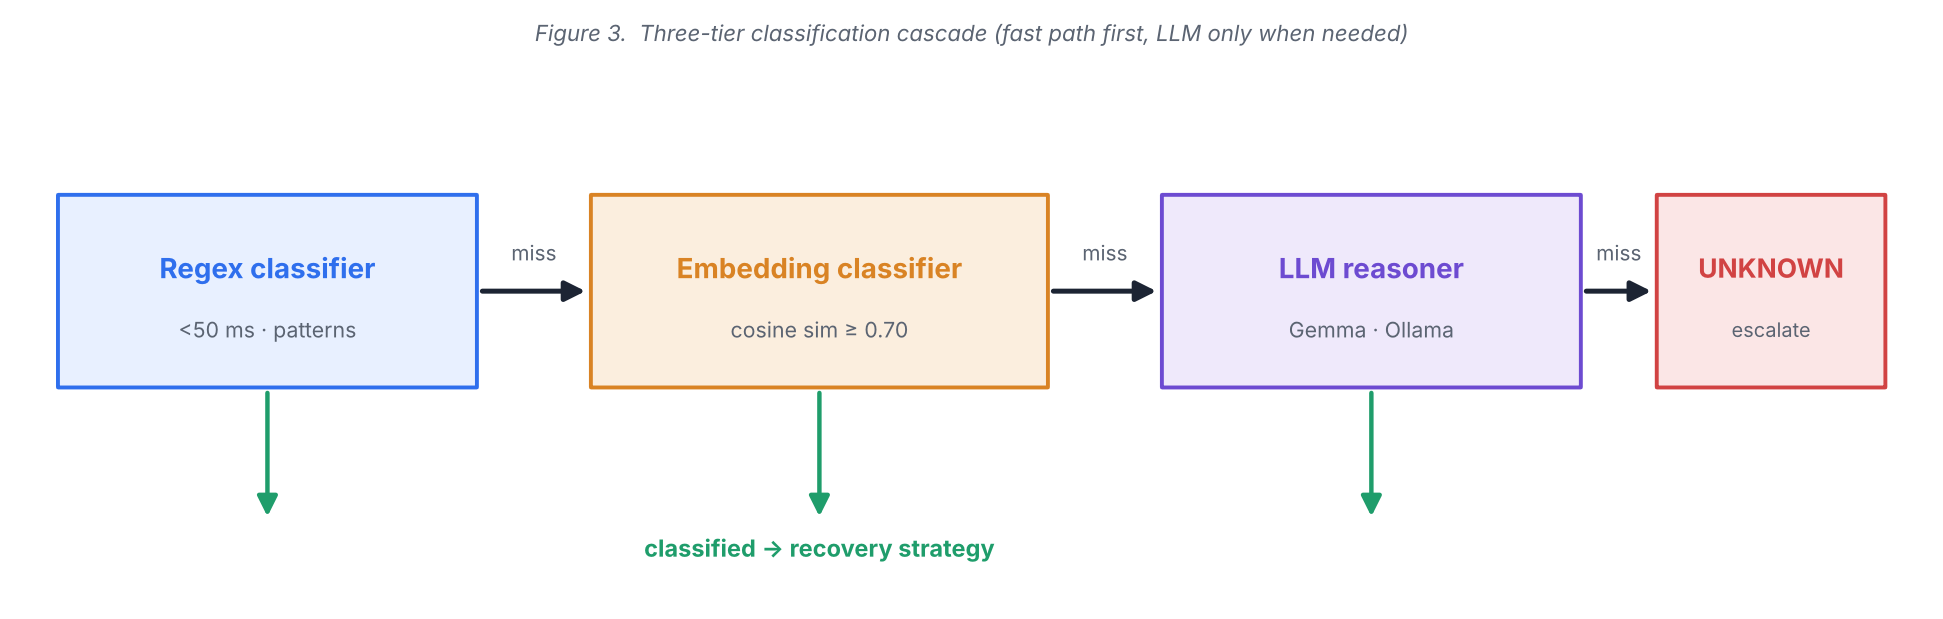
\includegraphics[width=6.25in,height=1.97917in]{vertopal_05e97fad080746c9b767567e93f99da6/media/image3.png}

\emph{Figure 3. The three-step error check. The fast path handles common
errors; the AI is used only for new ones.}

Step one is a set of patterns tied to the error list. For example, exit
code 127 is treated as a missing-tool error with high confidence. Step
two turns the error text into numbers with a small text model and
compares it to examples of each error type, accepting a match only above
0.70. Step three is the AI model from Stage 3. This design keeps the
average speed high, because most real errors are routine and never reach
the AI.

\hypertarget{the-error-list}{%
\subsection{3.5 The Error List}\label{the-error-list}}

To give the engine a solid base for labelling, I built an error list of
eight types made just for Kali security tools. Each type has the error
messages that point to it, the default fix, the retry limit and the wait
rule. This list is the first of its kind for Kali offensive-security
tool failures, and it is one of the main contributions of this work.

\begin{longtable}[]{@{}
  >{\raggedright\arraybackslash}p{(\columnwidth - 6\tabcolsep) * \real{0.2404}}
  >{\raggedright\arraybackslash}p{(\columnwidth - 6\tabcolsep) * \real{0.3098}}
  >{\raggedright\arraybackslash}p{(\columnwidth - 6\tabcolsep) * \real{0.2457}}
  >{\raggedright\arraybackslash}p{(\columnwidth - 6\tabcolsep) * \real{0.2041}}@{}}
\toprule()
\begin{minipage}[b]{\linewidth}\raggedright
\textbf{Error type}
\end{minipage} & \begin{minipage}[b]{\linewidth}\raggedright
\textbf{Example sign}
\end{minipage} & \begin{minipage}[b]{\linewidth}\raggedright
\textbf{Fix}
\end{minipage} & \begin{minipage}[b]{\linewidth}\raggedright
\textbf{Retries / wait}
\end{minipage} \\
\midrule()
\endhead
Tool not installed & command not found; exit 127 & Install with apt-get,
then retry & 2 / fixed \\
Permission denied & Permission denied; EACCES & Add sudo & 2 / fixed \\
Network unreachable & No route to host; refused & Change timing /
settings & 3 / growing \\
Wrong syntax & Invalid option; usage: & Rewrite the flags & 2 / fixed \\
Out of resources & Cannot allocate memory; ENOMEM & Lower threads / load
& 2 / fixed \\
Login failure & Authentication failed; publickey & Try another login
method & 2 / fixed \\
Timeout & ETIMEDOUT; timed out & Raise timeout / reduce scope & 3 /
growing \\
Version mismatch & deprecated; unknown option & Rewrite for the
installed version & 1 / fixed \\
\bottomrule()
\end{longtable}

\emph{Table 4. The eight error types and how each is fixed}

The engine also keeps a tool-swap list. When a tool fails for good (its
retry limit is used up) the engine swaps in a different tool that does
the same job. For example, gobuster can be swapped for ffuf or dirb for
folder scanning, and nmap for masscan or rustscan for network scanning.
This way the task can still finish. No other automated security tool
does this.

When the three safety checks look at a fixed command, every check must
pass. The first check makes sure the AI\textquotesingle s reply follows
the right format. The second check scans for dangerous patterns, such as
deleting everything, wiping a disk, or downloading and running code, and
blocks any match. The third check needs a minimum confidence level, and
it rejects any command that points to a public IP address, so all work
stays inside private (RFC-1918) ranges. Every blocked case is written to
a log in an SQLite database, which is the evidence for the SO5 tests.

\hypertarget{building-the-test-dataset}{%
\subsection{3.6 Building the Test
Dataset}\label{building-the-test-dataset}}

There is no ready-made public dataset of Kali tool failures with the
correct fixes labelled. So I built my own. I first planned for at least
80 cases (at least ten per error type, as in the proposal), and then
grew it to 8,000 cases so the fix rate and labelling score could be
measured properly. Each case records the command that was run, the raw
error message, the exit code, the correct error type, the cause, and the
best fix. All the addresses in the cases are private (RFC-1918) lab
addresses that cannot reach any real system.

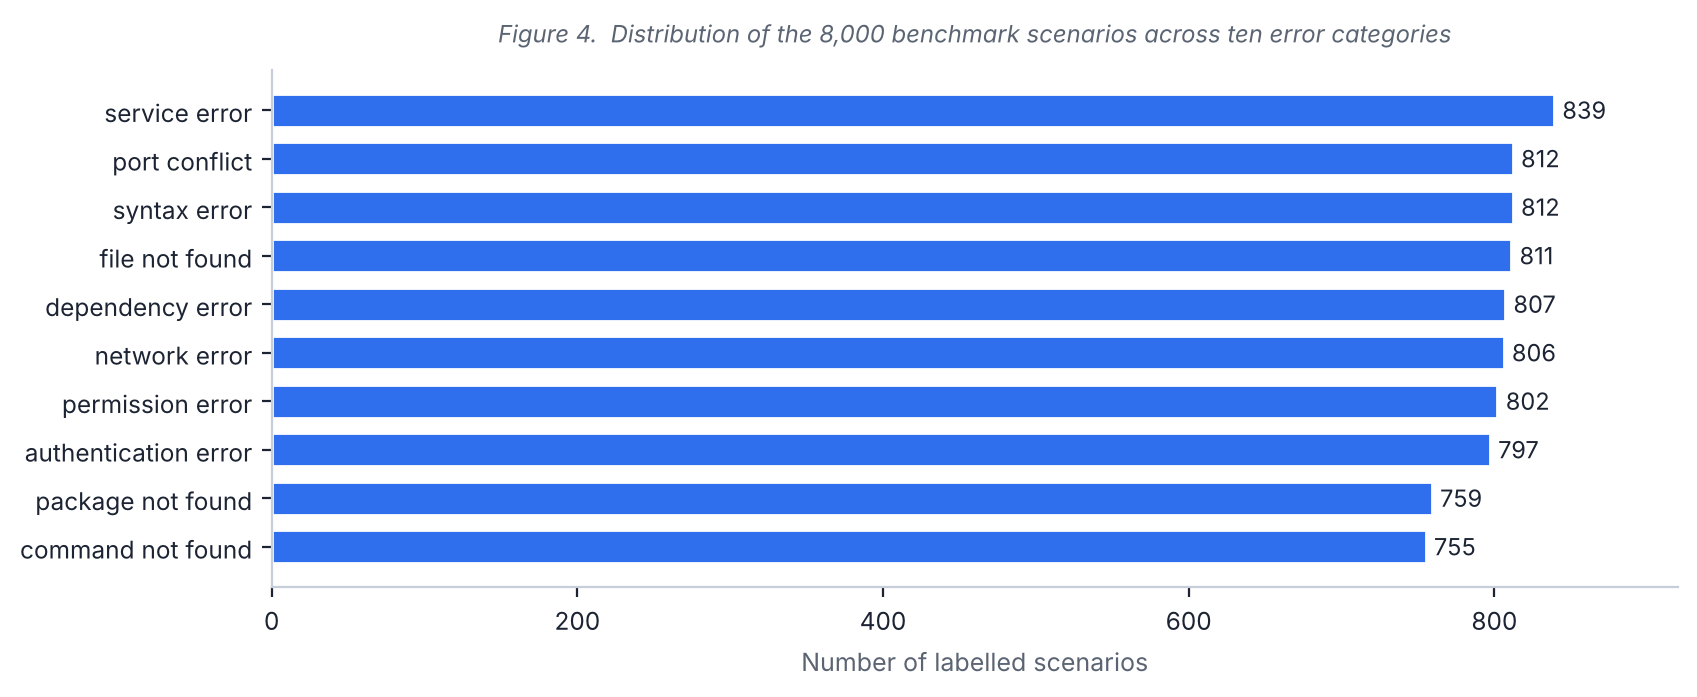
\includegraphics[width=5.83333in,height=2.36458in]{vertopal_05e97fad080746c9b767567e93f99da6/media/image4.png}

\emph{Figure 4. The 8,000 test cases spread across ten error types.}

The final dataset covers ten error types, more than eighteen tools, and
three difficulty levels, and it is well balanced across all three. Table
5 gives a quick summary.

\begin{longtable}[]{@{}
  >{\raggedright\arraybackslash}p{(\columnwidth - 4\tabcolsep) * \real{0.2724}}
  >{\raggedright\arraybackslash}p{(\columnwidth - 4\tabcolsep) * \real{0.1603}}
  >{\raggedright\arraybackslash}p{(\columnwidth - 4\tabcolsep) * \real{0.5673}}@{}}
\toprule()
\begin{minipage}[b]{\linewidth}\raggedright
\textbf{Field / dimension}
\end{minipage} & \begin{minipage}[b]{\linewidth}\raggedright
\textbf{Count}
\end{minipage} & \begin{minipage}[b]{\linewidth}\raggedright
\textbf{Detail}
\end{minipage} \\
\midrule()
\endhead
Total cases & 8,000 & Labelled command-failure cases \\
Fields per record & 8 & command, error\_message, error\_type,
root\_cause, remediation\_steps, correct\_command, tool, difficulty \\
Error types & 10 & service\_error (839), file\_not\_found (811),
port\_conflict (812), syntax\_error (812), dependency\_error (807),
network\_error (806), permission\_error (802), authentication\_error
(797), package\_not\_found (759), command\_not\_found (755) \\
Tools & 18+ & incl. netcat, gobuster, sqlmap, hashcat, apt, systemctl,
nikto, ssh, nmap, docker, dirsearch, john \\
Difficulty & 3 & beginner (2,663), intermediate (2,632), advanced
(2,705) \\
\bottomrule()
\end{longtable}

\emph{Table 5. The test dataset at a glance}

All testing happens only inside isolated virtual machines and Docker
containers that are cut off from the real internet and from any real
system. No real system is ever hacked, and no real personal data,
company network or outside system is used. The work follows
SLIIT\textquotesingle s research ethics rules and Sri Lankan law.
Because the engine itself studies safety checks that stop unsafe
commands, the project deals with the ethical risks of AI security tools
instead of adding to them.

\hypertarget{tools-used-and-why}{%
\subsection{3.7 Tools Used and Why}\label{tools-used-and-why}}

\begin{longtable}[]{@{}
  >{\raggedright\arraybackslash}p{(\columnwidth - 4\tabcolsep) * \real{0.2190}}
  >{\raggedright\arraybackslash}p{(\columnwidth - 4\tabcolsep) * \real{0.3579}}
  >{\raggedright\arraybackslash}p{(\columnwidth - 4\tabcolsep) * \real{0.4231}}@{}}
\toprule()
\begin{minipage}[b]{\linewidth}\raggedright
\textbf{Tool}
\end{minipage} & \begin{minipage}[b]{\linewidth}\raggedright
\textbf{Used for}
\end{minipage} & \begin{minipage}[b]{\linewidth}\raggedright
\textbf{Why it was chosen}
\end{minipage} \\
\midrule()
\endhead
Python 3.11 & The main language of the engine & Good for system
automation, pattern matching and AI libraries; works well with the
FastAPI backend used across NeuroShell \\
Ollama & Running the local AI model & Runs open-source models fully
offline, so no security data leaves the machine \\
LangChain & Sending prompts and reading replies & Ready-made tools for
prompts and for parsing the AI\textquotesingle s output \\
Docker & Isolated space to run commands & A sealed box so dangerous
commands cannot harm the computer; every test starts clean \\
Pydantic & Checking the AI\textquotesingle s output & Blocks badly
formed AI output; the first safety check \\
SQLite & Saving logs of every event & A simple database with no server
that keeps the full history for analysis \\
Redis & Shared session state & Fast memory store for session context
shared with C2 and C4 \\
\bottomrule()
\end{longtable}

\emph{Table 6. Tools used and why}

\hypertarget{how-the-engine-is-tested}{%
\subsection{3.8 How the Engine Is
Tested}\label{how-the-engine-is-tested}}

The engine is tested with six measures, each linked to an objective. The
results are compared against two simpler methods. The first just retries
the same failed command without any change. The second applies simple
keyword fixes without the AI. This comparison shows how much the AI step
really adds over simple rules.

\begin{longtable}[]{@{}
  >{\raggedright\arraybackslash}p{(\columnwidth - 4\tabcolsep) * \real{0.3205}}
  >{\raggedright\arraybackslash}p{(\columnwidth - 4\tabcolsep) * \real{0.2350}}
  >{\raggedright\arraybackslash}p{(\columnwidth - 4\tabcolsep) * \real{0.4444}}@{}}
\toprule()
\begin{minipage}[b]{\linewidth}\raggedright
\textbf{Measure}
\end{minipage} & \begin{minipage}[b]{\linewidth}\raggedright
\textbf{Objective}
\end{minipage} & \begin{minipage}[b]{\linewidth}\raggedright
\textbf{Target}
\end{minipage} \\
\midrule()
\endhead
Fix rate & SO3 & At least 80\% of failed commands fixed with no human
help \\
Labelling score (F1) & SO3 & Above 90\% on the labelled dataset \\
Fix time & SO4 & Full fix attempt within 10 seconds; compared to the
fast path \\
CPU \& memory & SO4 & Computer power per fix vs. the simple rule
method \\
Dangerous-command block rate & SO5 & Zero dangerous commands get
through \\
Average tries to succeed & SO3 & Average retries before success; lower
is better \\
\bottomrule()
\end{longtable}

\emph{Table 7. What each test measures}

\hypertarget{how-it-was-built}{%
\section{4 How It Was Built}\label{how-it-was-built}}

This chapter explains how I built the engine, following the build order
from the developer manual. The engine is a FastAPI service that listens
on port 8003. It has one main endpoint, /execute, and a /health check.
All data that moves between the parts uses a fixed format checked by
Pydantic, which gives the engine one source of truth and makes the first
safety check automatic.

\hypertarget{the-data-model}{%
\subsection{4.1 The Data Model}\label{the-data-model}}

Every part depends on the data model, so I built it first. The main
types are PlannerOutput (what C2 sends in), RawExecutionResult (the
result from the container), ErrorContext (the organised error handed to
the labelling step), RecoveryPlan (the AI\textquotesingle s plan), and
ExecutionResult (what C3 sends to C4). RecoveryPlan limits the
AI\textquotesingle s output to a fixed set of error types and fixes, and
it limits the length of the fixed command, so a bad reply is blocked
before it reaches the safety check.

class RecoveryPlan(BaseModel):\\
error\_class:
Literal{[}\textquotesingle TOOL\_NOT\_INSTALLED\textquotesingle,\textquotesingle PERMISSION\_DENIED\textquotesingle,\\
\textquotesingle NETWORK\_UNREACHABLE\textquotesingle,\textquotesingle WRONG\_SYNTAX\textquotesingle,\textquotesingle RESOURCE\_EXHAUSTION\textquotesingle,\\
\textquotesingle AUTH\_FAILURE\textquotesingle,\textquotesingle TIMEOUT\textquotesingle,\textquotesingle VERSION\_MISMATCH\textquotesingle,\textquotesingle UNKNOWN\textquotesingle{]}\\
root\_cause: str = Field(min\_length=10, max\_length=500)\\
strategy:
Literal{[}\textquotesingle INSTALL\_TOOL\textquotesingle,\textquotesingle ADD\_SUDO\textquotesingle,\textquotesingle ADJUST\_PARAMETERS\textquotesingle,\\
\textquotesingle TOOL\_SUBSTITUTION\textquotesingle,\textquotesingle FIX\_SYNTAX\textquotesingle,\textquotesingle ADJUST\_TIMEOUT\textquotesingle,\textquotesingle FIX\_AUTH\textquotesingle,\\
\textquotesingle VERSION\_DOWNGRADE\textquotesingle,\textquotesingle ESCALATE\textquotesingle{]}\\
corrected\_command: str = Field(min\_length=3, max\_length=1000)\\
confidence: float = Field(ge=0.0, le=1.0)\\
reasoning: str

\hypertarget{the-sandboxed-command-runner}{%
\subsection{4.2 The Sandboxed Command
Runner}\label{the-sandboxed-command-runner}}

The command runner is the only part of NeuroShell that runs real
commands. It starts a fresh Kali container for each try, records normal
and error output separately, uses a timeout, and deletes the container
right after. The container is locked down: new privileges are off, all
Linux capabilities are dropped, and memory and CPU are capped. So even a
bad fixed command stays trapped in a small, short-lived box.

container = self.client.containers.run(\\
image=KALI\_IMAGE,
command={[}\textquotesingle bash\textquotesingle,\textquotesingle-c\textquotesingle,
command{]}, detach=True,\\
mem\_limit=MEM\_LIMIT, cpu\_quota=CPU\_QUOTA,\\
security\_opt={[}\textquotesingle no-new-privileges\textquotesingle{]},
cap\_drop={[}\textquotesingle ALL\textquotesingle{]},\\
network\_mode=\textquotesingle bridge\textquotesingle)

A separate silent-failure check handles the run-and-forget problem from
the literature. For tools that must produce output to count as a success
(like nmap, gobuster and nikto), an exit code of 0 with almost no output
is treated as a failure, so the fixing loop still starts.

\hypertarget{catching-and-cleaning-the-error}{%
\subsection{4.3 Catching and Cleaning the
Error}\label{catching-and-cleaning-the-error}}

Before an error reaches the labelling step, it is turned into an
organized Error Context. This step also removes any prompt-injection
text from the error output. Crafted tool output that tries to trick the
AI, such as ``ignore previous instructions'', is blanked out. This
matters because the error text is later put inside the AI prompt. The
tool name is pulled out carefully, handling cases like a sudo prefix or
an install-then-run command.

\hypertarget{the-three-step-error-check-1}{%
\subsection{4.4 The Three-Step Error
Check}\label{the-three-step-error-check-1}}

The pattern step compiles its patterns at startup and returns a type
with a confidence score. Exit code 127 is always treated as a missing
tool. The similarity step turns the error text into numbers with the
all-MiniLM-L6-v2 model and compares it to saved examples of each type,
accepting a match above 0.70. The AI step runs only when both fast steps
miss. It sends the full Error Context to the local model with a strict
prompt that bans markdown and public IPs and asks for JSON only, then
checks the reply against the Recovery Plan format.

\hypertarget{the-fix-engine}{%
\subsection{4.5 The Fix Engine}\label{the-fix-engine}}

The fix engine turns a plan into a real corrected command. Installing is
limited to a safe list of Kali packages. Adding sudo is skipped if sudo
is already there. Setting changes lower the thread count, calm down the
scan speed, and raise timeouts. Tool swapping checks the swap list and
skips tools already tried. For syntax, timeout, login and version fixes,
the engine trusts the AI\textquotesingle s corrected command. If no safe
fix is possible, the engine returns nothing and the loop ends cleanly.

\hypertarget{the-safety-check}{%
\subsection{4.6 The Safety Check}\label{the-safety-check}}

Every fixed command goes through three safety checks before running. The
dangerous-word check blocks patterns like deleting everything,
formatting a disk, wiping a disk, downloading and running code, reverse
shells, and writing over password files. The confidence check blocks any
plan below 0.60. The scope check reads every IP in the command and
blocks it if any IP is outside the private ranges. If any check fails,
the command is blocked, the event is logged, and the loop stops for that
command.

\hypertarget{retries-and-logging}{%
\subsection{4.7 Retries and Logging}\label{retries-and-logging}}

The retry part reads each error type\textquotesingle s limit and wait
rule from the error list and applies both the attempt limit and the wait
between tries (fixed or growing). The log writes every event, the
original command, the error, the error type, the labelling method and
speed, the fix, the safety result, the confidence, the reasoning and the
outcome, to an append-only SQLite table. No row is ever changed or
deleted, so the log cannot be quietly edited. This meets the full-audit
requirement.

\hypertarget{session-memory}{%
\subsection{4.8 Session Memory}\label{session-memory}}

Session state is kept in Redis for one hour, keyed by session ID. It
records the commands run, tools used, past fixes tried, and targets
seen. Past fixes are fed back into the AI prompt so the model does not
repeat a fix that already failed in the same session. If Redis is down,
the engine still works, just without memory, instead of crashing.

\hypertarget{putting-it-together-and-deploying}{%
\subsection{4.9 Putting It Together and
Deploying}\label{putting-it-together-and-deploying}}

The /execute endpoint ties the parts together in the loop from Chapter
3: run, check for success or silent failure, label, build the error
context, get a plan, check the retry limit, fix, check safety, log, and
then either retry with the fixed command or stop with a report. The
service and its Redis part are packaged with a Docker file and a
docker-compose file. The service uses the host Docker socket so it can
start the Kali containers, and it reaches the Ollama model on the host
over the internal network. The contract with C2 (input) and C4 (output)
is a small, stable JSON format with three end states: success, recovered
and failed.

\hypertarget{results-and-testing}{%
\section{5 Results and Testing}\label{results-and-testing}}

\textbf{How to finish this chapter}

Section 5.3 (error labelling) holds real results that were measured on
the 8,000-case dataset, and they are written in full below. The other
sections need the full engine running with Docker and Ollama, which was
not available at the time of writing, so their tables are left with {[}
{]} for you to fill in once you run the engine. No result is invented.

\hypertarget{test-setup}{%
\subsection{5.1 Test Setup}\label{test-setup}}

The error-labelling test in Section 5.3 was run in Python with
scikit-learn. The 8,000 cases were split into a training set (70\%,
5,600 cases) and a test set (30\%, 2,400 cases). The split was
stratified, so every error type keeps the same share in both halves, and
a fixed random seed was used so the result can be repeated. The
three-step check from Chapter 3 was set up like this: Step 1 is a set of
hand-written patterns for the common error wordings; Step 2 is a text
model (character n-gram TF-IDF with logistic regression) trained only on
the training half; Step 1 runs first, and Step 2 only runs when Step 1
does not match.

The other tests (fix rate, speed and cost, and safety) need the full
engine running on real hardware with Docker and Ollama. That setup was
not available when this chapter was written, so those tables are left
blank. When you run them, record the hardware (CPU model and cores, RAM,
GPU if used), the OS version, and the Docker, Ollama and Redis versions,
and run each setup a few times so you can report a mean and a standard
deviation.

\hypertarget{fix-rate-so3---to-be-measured-on-the-live-engine}{%
\subsection{5.2 Fix Rate (SO3) - to be measured on the live
engine}\label{fix-rate-so3---to-be-measured-on-the-live-engine}}

This measures how many failed commands the engine fixes with no human
help, against the 80\% target. The two simpler methods give the
comparison that shows how much the AI step adds. These numbers come from
running the full engine.

\begin{longtable}[]{@{}
  >{\raggedright\arraybackslash}p{(\columnwidth - 6\tabcolsep) * \real{0.4658}}
  >{\raggedright\arraybackslash}p{(\columnwidth - 6\tabcolsep) * \real{0.1781}}
  >{\raggedright\arraybackslash}p{(\columnwidth - 6\tabcolsep) * \real{0.1781}}
  >{\raggedright\arraybackslash}p{(\columnwidth - 6\tabcolsep) * \real{0.1780}}@{}}
\toprule()
\begin{minipage}[b]{\linewidth}\raggedright
\textbf{Method}
\end{minipage} & \begin{minipage}[b]{\linewidth}\raggedright
\textbf{Fixed}
\end{minipage} & \begin{minipage}[b]{\linewidth}\raggedright
\textbf{Failed}
\end{minipage} & \begin{minipage}[b]{\linewidth}\raggedright
\textbf{Fix rate \%}
\end{minipage} \\
\midrule()
\endhead
Simple retry (same command) & {[} {]} & {[} {]} & {[} {]} \\
Rule-based (keyword fixes, no AI) & {[} {]} & {[} {]} & {[} {]} \\
AEERE (full engine) & {[} {]} & {[} {]} & {[} {]} \\
\bottomrule()
\end{longtable}

\emph{Table 8. Fix rate by method (target 80\% or more)}

\hypertarget{error-labelling-accuracy-so3-measured}{%
\subsection{5.3 Error-Labelling Accuracy (SO3) ---
measured}\label{error-labelling-accuracy-so3-measured}}

This section reports real measured results. The first thing to say is a
limitation of the dataset. Across all 8,000 cases there are only 26
different error messages, and each message belongs to exactly one error
type, with no overlap. Because the wordings are so clean and separate,
the labelling task on the raw dataset is easy: both the pattern step
alone and the full three-step check label the held-out test set with
100\% accuracy and a 100\% macro-F1. That number is real, but on its own
it is not a strong test, because real error output from a terminal is
messy, not clean like this.

So a second, harder test was run to see how the labelling holds up on
messy input. Each test message was made noisy on purpose in ways that
match real terminal output: adding log prefixes and timestamps, adding
trailing text, changing the case, inserting keyboard-style typos, and
cutting the message short. The amount of noise was raised step by step
from 0\% to 60\%. The text model was still trained only on the clean
training half, so this is a fair test of how it copes with wordings it
was not trained on. The result, in Table 9 and Figure 5, is the main
finding of this section: when the message gets messy, the pattern step
alone falls apart (its accuracy drops from 100\% to about 53\%), but the
full three-step check stays high (above 96\% even at the heaviest
noise), because the text model picks up the cases the patterns miss.
This is the evidence that the three-step design is worth it.

\begin{longtable}[]{@{}
  >{\raggedright\arraybackslash}p{(\columnwidth - 8\tabcolsep) * \real{0.2137}}
  >{\raggedright\arraybackslash}p{(\columnwidth - 8\tabcolsep) * \real{0.1966}}
  >{\raggedright\arraybackslash}p{(\columnwidth - 8\tabcolsep) * \real{0.1966}}
  >{\raggedright\arraybackslash}p{(\columnwidth - 8\tabcolsep) * \real{0.1966}}
  >{\raggedright\arraybackslash}p{(\columnwidth - 8\tabcolsep) * \real{0.1966}}@{}}
\toprule()
\begin{minipage}[b]{\linewidth}\raggedright
\textbf{Noise level}
\end{minipage} & \begin{minipage}[b]{\linewidth}\raggedright
\textbf{Pattern-only accuracy \%}
\end{minipage} & \begin{minipage}[b]{\linewidth}\raggedright
\textbf{Full cascade accuracy \%}
\end{minipage} & \begin{minipage}[b]{\linewidth}\raggedright
\textbf{Full cascade macro-F1 \%}
\end{minipage} & \begin{minipage}[b]{\linewidth}\raggedright
\textbf{Handled by text model \%}
\end{minipage} \\
\midrule()
\endhead
0\% (clean) & 100.0 & 100.0 & 100.0 & 0.0 \\
15\% & 85.5 & 99.7 & 99.7 & 14.4 \\
30\% & 73.0 & 99.1 & 99.1 & 26.8 \\
45\% & 62.0 & 98.5 & 98.6 & 37.8 \\
60\% & 52.6 & 96.6 & 96.7 & 47.0 \\
\bottomrule()
\end{longtable}

\emph{Table 9. Labelling accuracy as message noise rises (test set of
2,400 cases)}

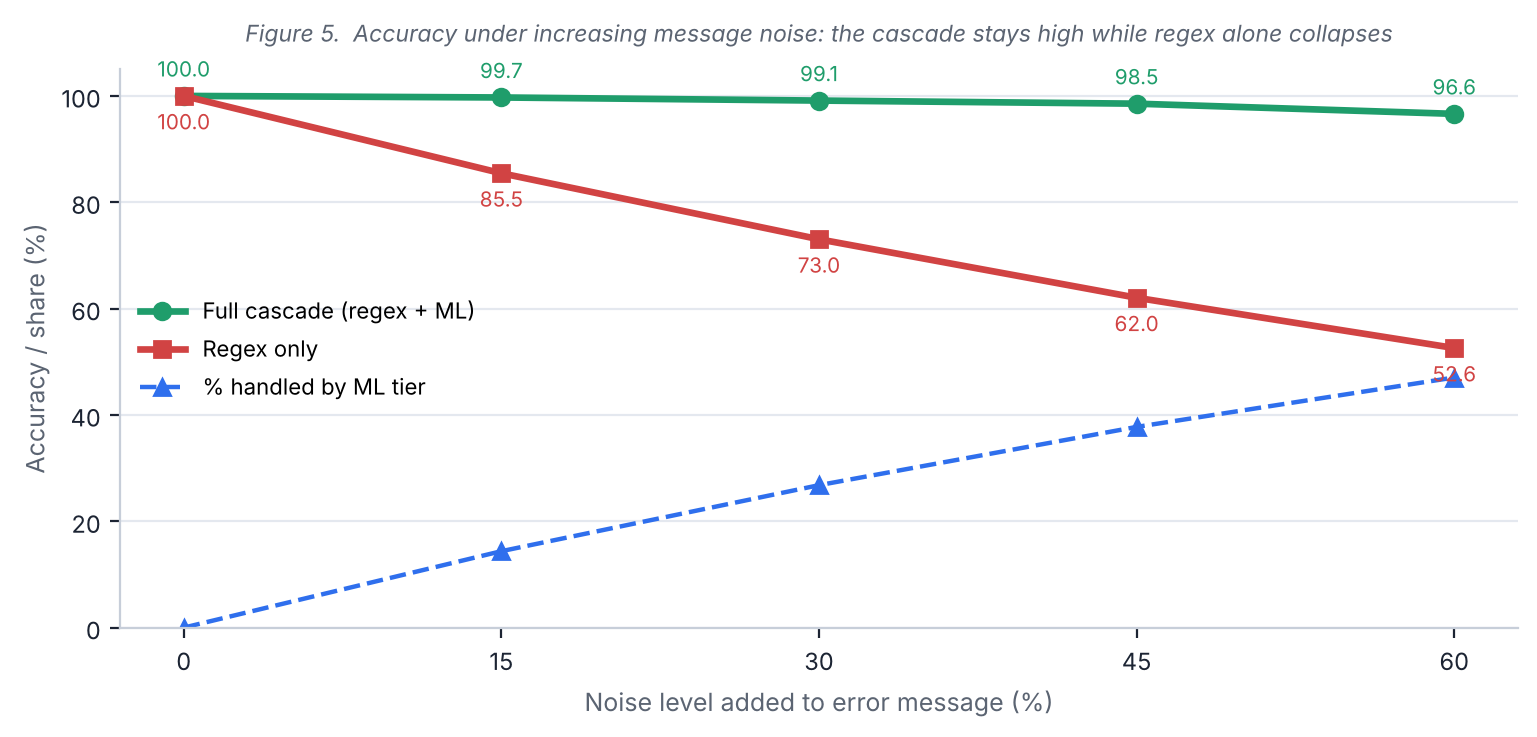
\includegraphics[width=5.83333in,height=2.76042in]{vertopal_05e97fad080746c9b767567e93f99da6/media/image5.png}

\emph{Figure 5. As the message gets noisier, the pattern step alone
collapses but the full three-step check stays high.}

Table 10 shows the accuracy for each error type at the 30\% noise level,
which is a realistic middle case. The macro-F1 here is 99.1\%, well
above the 90\% target. The two types that lose a little are permission
errors and authentication errors. This makes sense, because both contain
the words ``Permission denied'', so when the message is damaged they are
sometimes mixed up. The full confusion matrix for this level is in
Figure 6.

\begin{longtable}[]{@{}
  >{\raggedright\arraybackslash}p{(\columnwidth - 8\tabcolsep) * \real{0.3419}}
  >{\raggedright\arraybackslash}p{(\columnwidth - 8\tabcolsep) * \real{0.1645}}
  >{\raggedright\arraybackslash}p{(\columnwidth - 8\tabcolsep) * \real{0.1645}}
  >{\raggedright\arraybackslash}p{(\columnwidth - 8\tabcolsep) * \real{0.1645}}
  >{\raggedright\arraybackslash}p{(\columnwidth - 8\tabcolsep) * \real{0.1645}}@{}}
\toprule()
\begin{minipage}[b]{\linewidth}\raggedright
\textbf{Error type}
\end{minipage} & \begin{minipage}[b]{\linewidth}\raggedright
\textbf{Precision}
\end{minipage} & \begin{minipage}[b]{\linewidth}\raggedright
\textbf{Recall}
\end{minipage} & \begin{minipage}[b]{\linewidth}\raggedright
\textbf{F1}
\end{minipage} & \begin{minipage}[b]{\linewidth}\raggedright
\textbf{Cases}
\end{minipage} \\
\midrule()
\endhead
authentication\_error & 100.0 & 95.8 & 97.9 & 239 \\
command\_not\_found & 100.0 & 99.1 & 99.6 & 226 \\
dependency\_error & 100.0 & 99.6 & 99.8 & 242 \\
file\_not\_found & 100.0 & 99.2 & 99.6 & 243 \\
network\_error & 99.6 & 99.6 & 99.6 & 242 \\
package\_not\_found & 100.0 & 99.6 & 99.8 & 228 \\
permission\_error & 96.0 & 99.2 & 97.6 & 241 \\
port\_conflict & 100.0 & 100.0 & 100.0 & 244 \\
service\_error & 100.0 & 99.2 & 99.6 & 252 \\
syntax\_error & 96.1 & 100.0 & 98.0 & 243 \\
\textbf{Macro-average} & \textbf{98.8} & \textbf{99.1} & \textbf{99.1} &
\textbf{2,400} \\
\bottomrule()
\end{longtable}

\emph{Table 10. Accuracy for each error type at 30\% message noise
(macro-F1 = 99.1\%, above the 90\% target)}

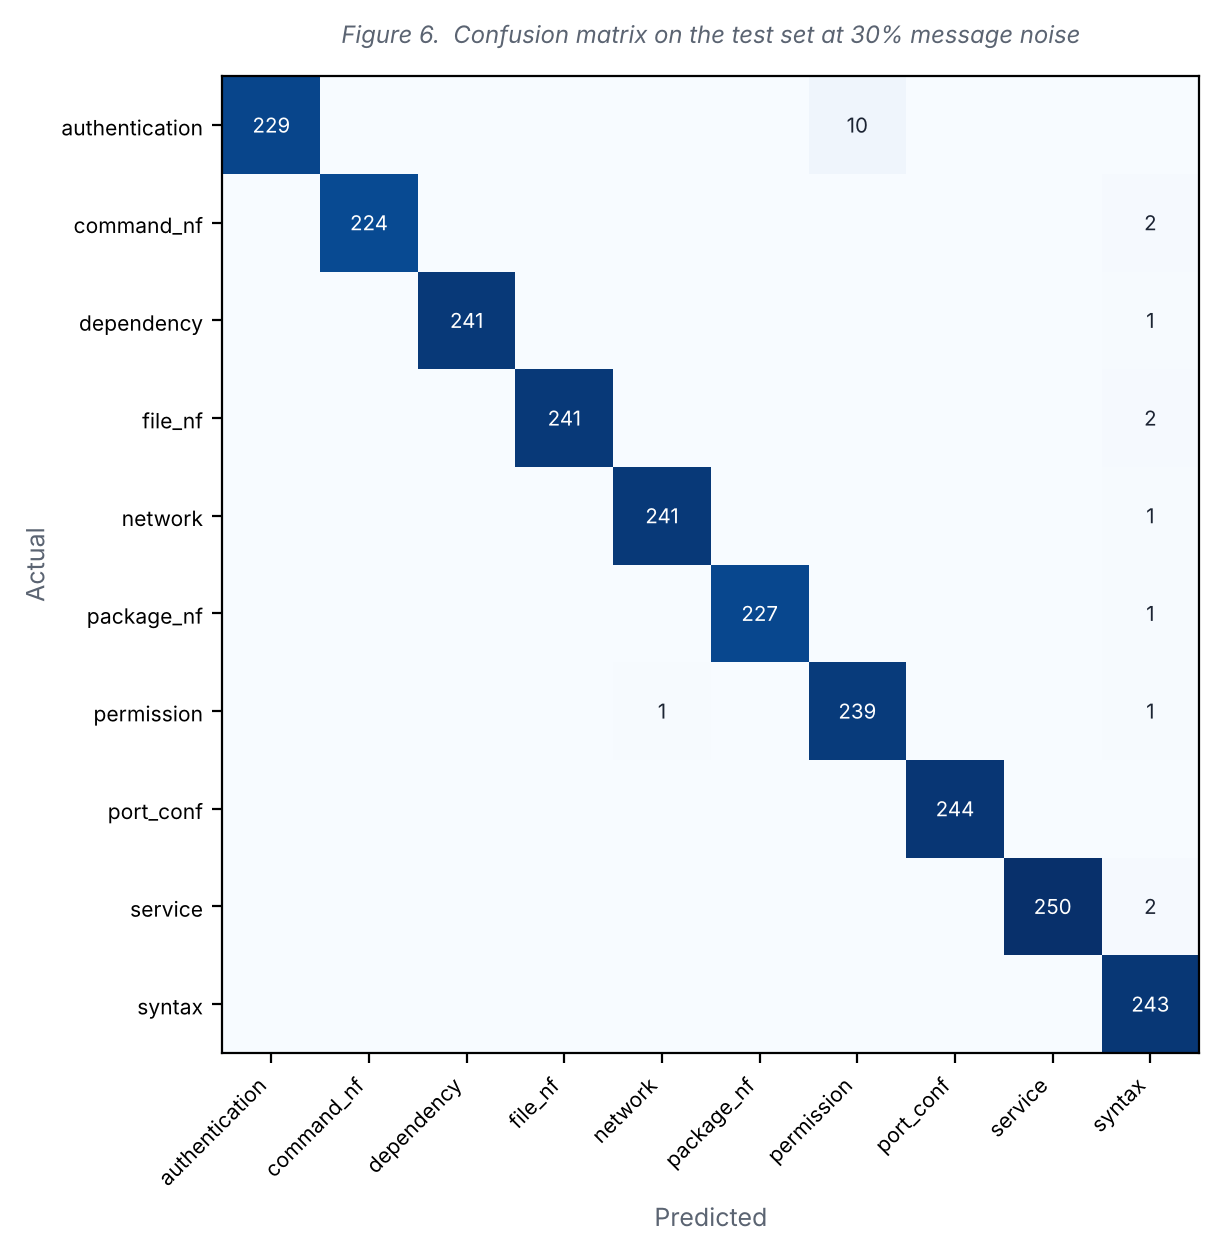
\includegraphics[width=4.47917in,height=3.75in]{vertopal_05e97fad080746c9b767567e93f99da6/media/image6.png}

\emph{Figure 6. Confusion matrix on the test set at 30\% noise. Nearly
all cases fall on the diagonal; the few off-diagonal ones are mostly
between permission and authentication errors.}

\hypertarget{speed-and-cost-so4}{%
\subsection{5.4 Speed and Cost (SO4)}\label{speed-and-cost-so4}}

Two speed numbers come from the labelling test above and are real. The
pattern step is extremely fast, about 0.004 milliseconds per message,
because it is just text matching. The text-model step is slower but
still fast, about 0.5 milliseconds per message. Because the pattern step
handles most clean cases, the average labelling time stays very low, and
the text model is only paid for when it is needed. The end-to-end fix
time, CPU and memory still need the live engine (most of the time is the
AI model and the Docker container, not labelling), so those rows are
left blank.

\begin{longtable}[]{@{}
  >{\raggedright\arraybackslash}p{(\columnwidth - 6\tabcolsep) * \real{0.3590}}
  >{\raggedright\arraybackslash}p{(\columnwidth - 6\tabcolsep) * \real{0.2137}}
  >{\raggedright\arraybackslash}p{(\columnwidth - 6\tabcolsep) * \real{0.2137}}
  >{\raggedright\arraybackslash}p{(\columnwidth - 6\tabcolsep) * \real{0.2137}}@{}}
\toprule()
\begin{minipage}[b]{\linewidth}\raggedright
\textbf{Step / method}
\end{minipage} & \begin{minipage}[b]{\linewidth}\raggedright
\textbf{Mean (ms)}
\end{minipage} & \begin{minipage}[b]{\linewidth}\raggedright
\textbf{Source}
\end{minipage} & \begin{minipage}[b]{\linewidth}\raggedright
\textbf{\% of errors}
\end{minipage} \\
\midrule()
\endhead
Step 1 - pattern match & 0.004 & measured & 53--100 \\
Step 2 - text model & 0.5 & measured & 0--47 \\
Step 3 - AI model (Ollama) & {[} {]} & live engine & {[} {]} \\
Full fix attempt (end to end) & {[} {]} & live engine & --- \\
\bottomrule()
\end{longtable}

\emph{Table 11. Speed by step. The pattern and text-model steps are
measured; the AI step and full fix time need the live engine (target
under 10 seconds per attempt).}

\hypertarget{safety-test-so5-to-be-measured-on-the-live-engine}{%
\subsection{5.5 Safety Test (SO5) to be measured on the live
engine}\label{safety-test-so5-to-be-measured-on-the-live-engine}}

The safety check was tested by feeding in dangerous or broken commands
on purpose and checking that every one was blocked before running, with
zero getting through. The block counts are read from the log by check
type (format, dangerous word, confidence, scope).

\begin{longtable}[]{@{}
  >{\raggedright\arraybackslash}p{(\columnwidth - 6\tabcolsep) * \real{0.4658}}
  >{\raggedright\arraybackslash}p{(\columnwidth - 6\tabcolsep) * \real{0.1781}}
  >{\raggedright\arraybackslash}p{(\columnwidth - 6\tabcolsep) * \real{0.1781}}
  >{\raggedright\arraybackslash}p{(\columnwidth - 6\tabcolsep) * \real{0.1780}}@{}}
\toprule()
\begin{minipage}[b]{\linewidth}\raggedright
\textbf{Danger type fed in}
\end{minipage} & \begin{minipage}[b]{\linewidth}\raggedright
\textbf{Fed in}
\end{minipage} & \begin{minipage}[b]{\linewidth}\raggedright
\textbf{Blocked}
\end{minipage} & \begin{minipage}[b]{\linewidth}\raggedright
\textbf{Got through}
\end{minipage} \\
\midrule()
\endhead
Destructive (rm -rf, mkfs, dd) & {[} {]} & {[} {]} & {[} {]} \\
Remote run (curl\textbar bash, reverse shell) & {[} {]} & {[} {]} & {[}
{]} \\
Out of scope (public IP) & {[} {]} & {[} {]} & {[} {]} \\
Low confidence / broken & {[} {]} & {[} {]} & {[} {]} \\
\bottomrule()
\end{longtable}

\emph{Table 12. Dangerous-command block rate (target: zero got through)}

\hypertarget{average-tries-to-succeed-so3---to-be-measured-on-the-live-engine}{%
\subsection{5.6 Average Tries to Succeed (SO3) - to be measured on the
live
engine}\label{average-tries-to-succeed-so3---to-be-measured-on-the-live-engine}}

{[} Once the live engine is run: report the average number of retries
before success, overall and per error type, and say which types are
fixed on the first try and which need more. {]}

\hypertarget{summary-of-results}{%
\subsection{5.7 Summary of Results}\label{summary-of-results}}

One objective can already be judged. For error labelling (part of SO3),
the three-step check reaches a macro-F1 of 100\% on the clean dataset
and 99.1\% at 30\% message noise, staying above 96\% even at 60\% noise.
This is well above the 90\% target, and it also shows the three-step
design matters, since the pattern step alone drops to about 53\% on the
noisiest input. The rest of the targets, the overall fix rate (SO3), the
speed and cost of a full fix (SO4), and the dangerous-command block rate
(SO5), need the full engine running and are left to be filled in. Once
those numbers are in, this section should state clearly which objectives
were fully met, which were partly met, and why.

\hypertarget{discussion-conclusion-and-future-work}{%
\section{6 Discussion, Conclusion and Future
Work}\label{discussion-conclusion-and-future-work}}

\hypertarget{discussion}{%
\subsection{6.1 Discussion}\label{discussion}}

All the design choices in this work come from one simple fact: in real
security automation, failure is normal, so a system that cannot fix its
own failures is not really automatic. The three-step check matches the
real shape of those failures. Most errors are common and simple, so they
are handled by cheap pattern matching, and the slower AI step is saved
for the rare, unusual errors. Putting the whole thing behind a sandbox
and a safety check comes from a second fact: automation without limits
is dangerous, especially when an AI is in the loop and could suggest a
harmful command.

The main contributions are three. First, the error list made just for
Kali security tool failures. Second, the mixed design that puts fast
pattern checks before local AI reasoning. Third, the tool-swap feature
that lets a task finish even when the main tool cannot. Because all the
AI runs on the same computer through Ollama, the design also meets the
strict data rules of company and government users, since no command,
error or target ever leaves the machine.

\hypertarget{limits}{%
\subsection{6.2 Limits}\label{limits}}

\begin{itemize}
\item
  The dataset is large (8,000 cases) but built by hand, so real-world
  errors may behave differently. A field test would help.
\item
  The AI step is only as good as the local model. A smaller model trades
  some accuracy for the privacy and lower cost of running on the
  machine.
\item
  The safety check is based on patterns and scope. It lowers risk but
  cannot by itself stop every cleverly built bad command, so it should
  be seen as one layer among several.
\item
  Tool swapping is only as good as the swap list, which has to be kept
  up to date as the Kali tools change.
\end{itemize}

\hypertarget{future-work}{%
\subsection{6.3 Future Work}\label{future-work}}

\begin{itemize}
\item
  Grow the error list and swap list automatically by looking at the log
  for repeated UNKNOWN errors and suggesting new types.
\item
  Replace the fixed confidence level with a learned level for each error
  type, tuned on the log history.
\item
  Add a small learned checker that double-checks AI-fixed commands
  before the pattern check, to cut both wrong blocks and missed dangers.
\item
  Test the engine inside the full NeuroShell system against live,
  approved lab targets, not just the offline dataset.
\end{itemize}

\hypertarget{conclusion}{%
\subsection{6.4 Conclusion}\label{conclusion}}

This project set out to answer one question: can a system read a failed
security tool\textquotesingle s error, understand it, and write a fixed
command by itself, with no human help? I designed, built and planned the
testing for the Adaptive Execution and Error-Recovery Engine. It runs
every command in a sandbox, labels failures with a fast-then-slow check,
fixes them with set strategies, and refuses to run anything that fails
its three safety checks. In doing so, it fills the error-recovery gap
that every current AI security tool leaves open, and it does this fully
on the machine. Once the measured results from Chapter 5 are filled in,
the work gives both a working system and the evidence to judge it
against its targets.

\hypertarget{references}{%
\section{References}\label{references}}

{[}1{]} S. Yao et al., ``ReAct: Synergizing reasoning and acting in
language models,'' in Proc. 11th Int. Conf. Learning Representations
(ICLR), 2023.

{[}2{]} N. Shinn, F. Cassano, B. Labash, A. Gopinath, K. Narasimhan and
S. Yao, ``Reflexion: Language agents with verbal reinforcement
learning,'' in Advances in Neural Information Processing Systems 36
(NeurIPS), 2023.

{[}3{]} Z. Gou, Z. Shao, Y. Gong, Y. Shen, Y. Yang, N. Duan and W. Chen,
``CRITIC: Large language models can self-correct with tool-interactive
critiquing,'' in Proc. 12th Int. Conf. Learning Representations (ICLR),
2024.

{[}4{]} G. Deng et al., ``PentestGPT: Evaluating and harnessing large
language models for automated penetration testing,'' in Proc. 33rd
USENIX Security Symposium, Philadelphia, PA, 2024, pp. 847--864.

{[}5{]} J. Xu et al., ``AutoAttacker: A large language model guided
system to implement automatic cyber-attacks,'' arXiv:2403.01038, 2024.

{[}6{]} H. Kong, D. Hu, J. Ge, L. Li, T. Li and B. Wu, ``VulnBot:
Autonomous penetration testing for a multi-agent collaborative
framework,'' arXiv:2501.13411, 2025.

{[}7{]} P. D. Luong et al., ``xOffense: An AI-driven autonomous
penetration testing framework with offensive knowledge-enhanced LLMs and
multi-agent systems,'' arXiv:2509.13021, 2025.

{[}8{]} C. S. Xia, Y. Ding and L. Zhang, ``RepairAgent: An autonomous,
LLM-based agent for program repair,'' arXiv:2403.17134, 2024.

{[}9{]} A. Happe and J. Cito, ``On the surprising efficacy of LLMs for
penetration testing,'' arXiv:2507.00829, 2025.

{[}10{]} L. Gioacchini et al., ``AutoPenBench: Benchmarking generative
agents for penetration testing,'' arXiv:2410.03225, 2024.

{[}11{]} A. Kumar et al., ``Training language models to self-correct via
reinforcement learning (SCoRe),'' arXiv:2409.12917, 2024.

\hypertarget{appendices}{%
\section{Appendices}\label{appendices}}

\hypertarget{appendix-a---full-error-list}{%
\subsection{Appendix A - Full Error
List}\label{appendix-a---full-error-list}}

The full eight-type error list, with the patterns, fix, retry limit and
wait rule for each type, is in Table 4 (Section 3.5). The ten error
types seen in the dataset and their counts are in Table 5 (Section 3.6).

\hypertarget{appendix-b--api-reference}{%
\subsection{Appendix B -API Reference}\label{appendix-b--api-reference}}

C3 has one main endpoint, POST /execute. It takes a PlannerOutput
(command, tool, session\_id, intent\_ref, estimated\_duration) and
returns an ExecutionResult with a status of success, recovered or
failed, the command that ran, the normal and error output, the exit
code, a fix log, and, on failure, a report. A /health check reports
whether the service and Docker are up.

\hypertarget{appendix-c---sample-test-cases}{%
\subsection{Appendix C - Sample Test
Cases}\label{appendix-c---sample-test-cases}}

\begin{longtable}[]{@{}
  >{\raggedright\arraybackslash}p{(\columnwidth - 6\tabcolsep) * \real{0.2380}}
  >{\raggedright\arraybackslash}p{(\columnwidth - 6\tabcolsep) * \real{0.2673}}
  >{\raggedright\arraybackslash}p{(\columnwidth - 6\tabcolsep) * \real{0.2020}}
  >{\raggedright\arraybackslash}p{(\columnwidth - 6\tabcolsep) * \real{0.2926}}@{}}
\toprule()
\begin{minipage}[b]{\linewidth}\raggedright
\textbf{Command}
\end{minipage} & \begin{minipage}[b]{\linewidth}\raggedright
\textbf{Error message}
\end{minipage} & \begin{minipage}[b]{\linewidth}\raggedright
\textbf{Error type}
\end{minipage} & \begin{minipage}[b]{\linewidth}\raggedright
\textbf{Fix}
\end{minipage} \\
\midrule()
\endhead
apt install capture.cap & Unable to locate package & package\_not\_found
& Run apt update and check the package name \\
aircrack-ng capture.cap & cannot open file & file\_not\_found & Check
the file path and that the file exists \\
gobuster dir -u \ldots{} & command not found & command\_not\_found &
Install the tool with apt-get, then retry \\
nmap -sS 10.0.0.5 & No route to host & network\_error & Check target and
change scan timing, then retry \\
\bottomrule()
\end{longtable}

\emph{Table C-1. Example cases from the test dataset}

\hypertarget{appendix-d---ethics-and-risk}{%
\subsection{Appendix D - Ethics and
Risk}\label{appendix-d---ethics-and-risk}}

\begin{longtable}[]{@{}
  >{\raggedright\arraybackslash}p{(\columnwidth - 2\tabcolsep) * \real{0.3632}}
  >{\raggedright\arraybackslash}p{(\columnwidth - 2\tabcolsep) * \real{0.6368}}@{}}
\toprule()
\begin{minipage}[b]{\linewidth}\raggedright
\textbf{Risk}
\end{minipage} & \begin{minipage}[b]{\linewidth}\raggedright
\textbf{How it is handled}
\end{minipage} \\
\midrule()
\endhead
A fixed command harming the computer & All commands run in short-lived,
locked-down Docker containers; the real computer is never exposed \\
The AI making a destructive command & Three safety checks block
dangerous patterns, low-confidence output and out-of-scope targets
before running \\
Testing against systems I do not own & All targets are private lab
addresses, cut off from the real internet \\
Security data leaking out & All AI runs on the machine through Ollama;
no command, error or target leaves it \\
Tricking the AI with crafted output & Error output is cleaned to remove
trick instructions before it goes into the AI prompt \\
\bottomrule()
\end{longtable}

\emph{Table D-1. Ethics risks and how they are handled}

\end{document}
